\documentclass[twoside,bibliography=totoc,openany]{fumi}

% Angaben zur Arbeit
\newcommand{\thesistitle}{Adaptive Lernverfahren: Systematisierung und didaktische Aufbereitung}
\newcommand{\thesisauthor}{Johannes Dankert}
\newcommand{\thesissupervidsor}{Dr. Niels Seidel}
\newcommand{\thesistype}{Bachelorarbeit}
\newcommand{\course}{Informatik}
\newcommand{\thesismatrikelnummer}{4279727}

\title{\thesistitle}
\author{\thesisauthor}
\date{\today}

% Von Pandoc erzeugte Kapitel verwenden dieses Kommando für kompakte Listen.
\providecommand{\tightlist}{%
  \setlength{\itemsep}{0pt}\setlength{\parskip}{0pt}}
\setlength{\emergencystretch}{3em}

\hyphenation{
  Lern-ressource
  Lern-ressourcen
  Lern-zustands-modellierung
  Adaptions-entscheidung
  Elo-Verfahren
  Auf-gaben-schwierig-keit
  Erfolgs-wahr-schein-lich-keit
}

\begin{document}
\sffamily
\pagestyle{empty}

%% Die erste Seite eines Buches
\thesisauthor\\{\textbf{\thesistitle}}\vfill\newpage~\newpage

%% Die Seite mit den Titelangaben
\vspace{2cm}
\begin{center}\LARGE
\vfill
{\Huge\thesistitle}\\
\vfill
\thesistype\\
im Studiengang \course
\vfill
eingereicht von\\[4pt]
\textbf{\thesisauthor}\\[4pt]
(Matrikelnummer \thesismatrikelnummer)\\
\vfill
angefertigt am\\
Lehrgebiet Kooperative Systeme\\
Fakultät Mathematik und Informatik\\
FernUniversität in Hagen\\
\vfill
Betreut durch\\
\thesissupervidsor
\vfill
\monthname[\the\month] \the\year
\end{center}
\newpage~\newpage

%% Leerseite mit Titel
{\large\textbf{\thesisauthor}\\\textbf{\thesistitle}\vfill}
\newpage~\newpage

%% Kurzfassungen
\section*{Zusammenfassung}
% !TEX root = ../main.tex

\textit{Platzhalter: Die deutschsprachige Kurzfassung wird nach
Fertigstellung der Arbeit ergänzt.}

\vfill
\section*{Summary}
% !TEX root = ../main.tex

\textit{Placeholder: The English abstract will be added after the thesis
has been completed.}

\vfill\newpage

%% Bibliografische Angaben
{\small
\thesisauthor. \textit{\thesistitle}. \thesistype.
Fakultät Mathematik und Informatik, FernUniversität in Hagen, \the\year.
\\\vfill

Diese Publikation ist unter \emph{Creative Commons -- Namensnennung 3.0 Deutschland}
lizenziert und darf als Ganzes oder ausschnittweise vervielfältigt, verbreitet und
öffentlich zugänglich gemacht werden, sofern dies im Text nicht anders vermerkt
ist.\newline\vspace{10pt}
\hspace{-9pt}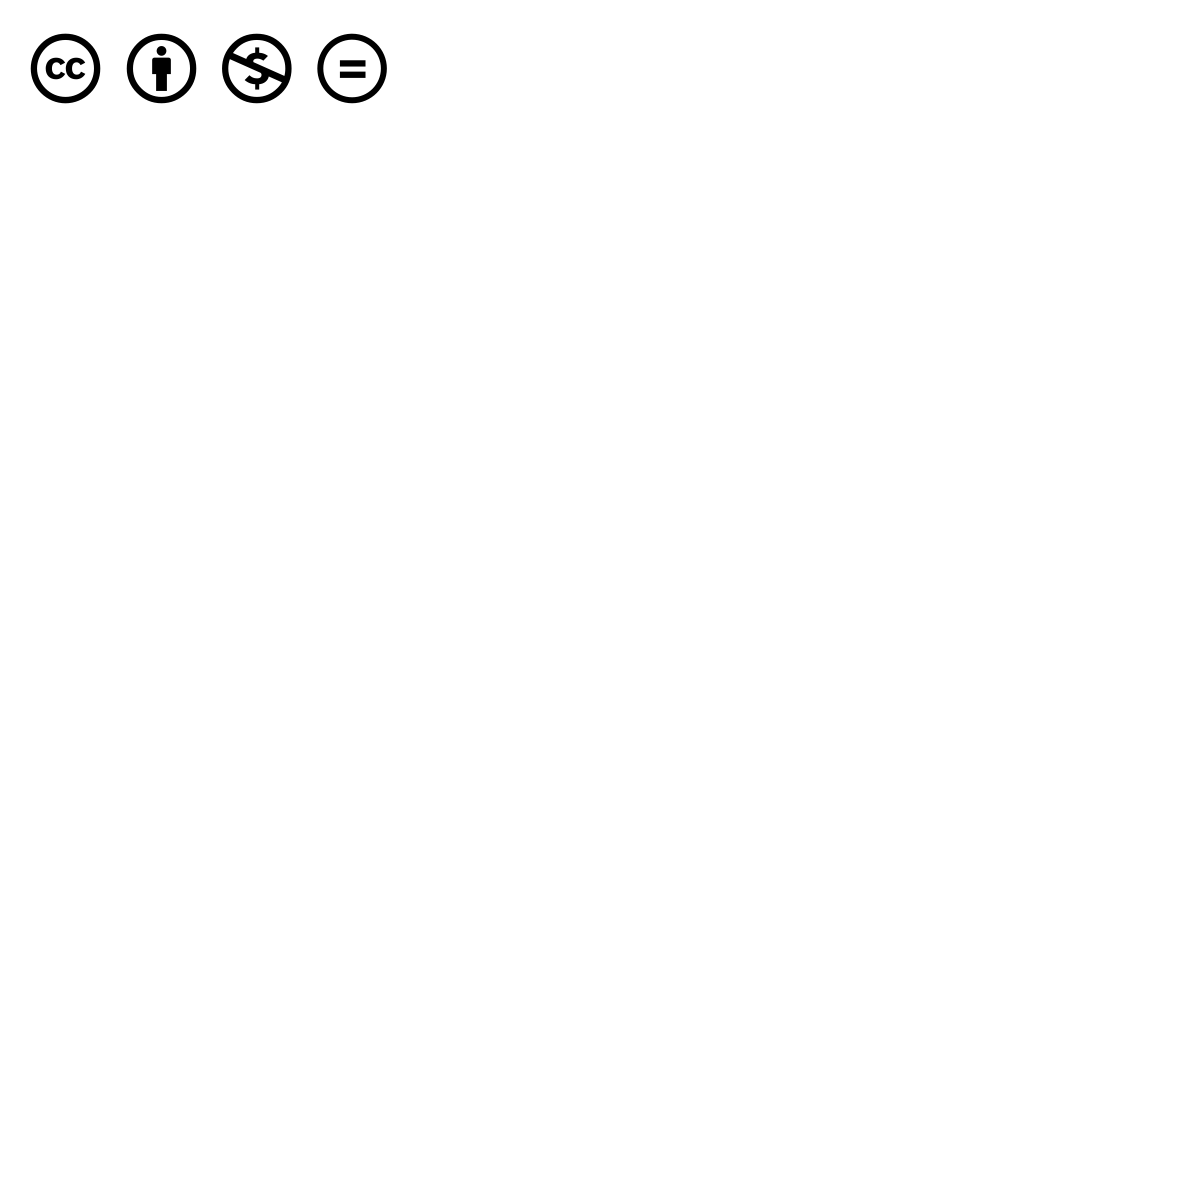
\includegraphics[height=10mm,viewport=0 1080 210 1200,clip]{logo-cc.png}
\\\vspace{10pt}

Autor: \thesisauthor\\
Gestaltung und Satz: \thesisauthor{} / \LaTeX\\
Datum: \today\\
\cleardoublepage
}

%% Inhaltsverzeichnis
\pagestyle{headings}
\tableofcontents

%% Hauptteil
\include{kapitel/01-einleitung}
% !TEX root = ../main.tex

\chapter{Analyse adaptiver
Lernverfahren}\label{analyse-adaptiver-lernverfahren}

\section{Forschungsstand und verwandte
Arbeiten}\label{forschungsstand-und-verwandte-arbeiten}

Die neuere Literatur beschreibt adaptive Lernsysteme nicht als einzelne,
klar umrissene Technologie, sondern als breites Feld personalisierter
digitaler Lernumgebungen, die Inhalte, Rückmeldungen, Aufgaben oder
Lernpfade auf Grundlage von Lernerdaten dynamisch anpassen
\citep{duPlooy2024, Wang2025, Martin2020}. Überblicksarbeiten
verdeutlichen dabei, dass adaptive Lernsysteme in sehr unterschiedlichen
Bildungskontexten - etwa in Hochschulumgebungen, intelligenten
Tutorensystemen oder digitalen Lernplattformen - eingesetzt werden und
zugleich methodisch stark ausdifferenzViert sind. Das Spektrum reicht von
klassischen psychometrischen und probabilistischen Modellen über
regelbasierte und wissensbasierte Verfahren bis hin zu
Recommender-Systemen sowie neueren KI- und Machine-Learning-Ansätzen
\citep{Wang2025, Hariyanto2025, daSilva2023, Liu2024}.\\
Adaptive Lerntechnologien lassen sich daher nicht auf einzelne
technische Ansätze reduzieren, sondern umfassen unterschiedliche
Verfahren, Modelle und Formen der Personalisierung.

Allgemeine Überblicksarbeiten betonen häufig die pädagogischen,
organisatorischen und implementierungsbezogenen Potenziale adaptiver
Lernsysteme. Für den Hochschulbereich zeigt ein aktueller Scoping
Review, dass adaptive Lernangebote häufig mit Verbesserungen von
Lernleistung und Engagement verbunden sind, zugleich jedoch durch
technische, zeitliche und organisatorische Ressourcen begrenzt werden.
Eine weitere Review zu KI-gestützten Adaptive-Learning-Plattformen hebt
hervor, dass insbesondere Plattformdesign, pädagogische Fundierung,
praktische Implementierung sowie geeignete Evaluationsmetriken zentrale
Themen des Forschungsfeldes darstellen. Solche Arbeiten machen die
Breite und Vielfalt adaptiver Lernsysteme deutlich, betrachten Verfahren
jedoch häufig primär auf Ebene konkreter Plattformen oder
Anwendungsszenarien. Die zugrunde liegenden algorithmischen Verfahren
werden dabei meist nicht systematisch als eigenständige
Verfahrensfamilien analysiert \citep{duPlooy2024, Tan2025}.

Daneben existieren zahlreiche spezialisierte Reviews, die jeweils nur
einzelne Teilbereiche adaptiver Lernsysteme untersuchen. Wang et
al.~analysieren adaptive E-Learning-Systeme mit Fokus auf die
Modellierung von Lernendenmerkmalen und die Verfahren zu deren
Identifikation. Die Autoren zeigen dabei insbesondere die große
methodische Vielfalt bestehender Learner-Modeling-Ansätze sowie eine
zunehmende Erweiterung des eingesetzten Methodenspektrums von
klassischen regelbasierten und probabilistischen Verfahren hin zu
breiteren Machine-Learning-Ansätzen \citep{Wang2025}. Desmarais und
Baker heben insbesondere probabilistische Modelle und Modelle latenter
Wissenszustände als zentrale Ansätze des Learner- und Skill-Modelings in
intelligenten Lernumgebungen hervor und zeigen, dass Verfahren zur
Wissensdiagnose eine Schlüsselrolle innerhalb adaptiver Systeme
einnehmen \citep{Desmarais2012}. Neuere Surveys zu Knowledge Tracing
beschreiben zudem einen Übergang von klassischen probabilistischen
Verfahren wie Bayesian Knowledge Tracing hin zu tiefen neuronalen
Sequenzmodellen \citep{Abdelrahman2023}. Im Bereich des Computerized
Adaptive Testing liegt der Fokus insbesondere auf Verfahren zur
adaptiven Auswahl informativer Testaufgaben sowie auf der
kontinuierlichen Fähigkeitsdiagnostik unter Verwendung psychometrischer
Modelle \citep{Han2018, Liu2024}. Aktuelle Reviews zu Reinforcement
Learning im Bildungsbereich zeigen, dass RL-Verfahren insbesondere zur
sequentiellen Optimierung adaptiver Lernentscheidungen eingesetzt
werden, zugleich jedoch weiterhin Herausforderungen hinsichtlich
realistischer Trainingsdaten und praktischer Implementierung bestehen
\citep{Riedmann2025}.\\
Der Forschungsstand ist damit reich an spezialisierten Teilanalysen,
enthält jedoch bislang nur wenige übergreifende Einordnungen, die
unterschiedliche Verfahrensfamilien systematisch und aus informatischer
Perspektive über Anwendungskontexte hinweg zusammenführen.

Darüber hinaus untersucht ein Teil der Literatur adaptive Lernsysteme
aus Perspektive von Implementierung, Akzeptanz und
Stakeholderbeteiligung. Alajlani, Crabb und Murray zeigen in ihrem
systematischen Review, dass Lehrende bislang nur in begrenztem Umfang in
Design, Implementierung und Evaluation adaptiver Lernsysteme eingebunden
sind \citep{Alajlani2024}. Diese Perspektive ist insbesondere für die
praktische Einführung adaptiver Lernsysteme relevant, trägt jedoch nur
eingeschränkt dazu bei, die zugrunde liegenden Verfahren und
Adaptionsmechanismen systematisch einzuordnen.

Insgesamt zeigt der Forschungsstand damit eine deutliche
Perspektivenpluralität: Pädagogische, didaktische, organisationale,
anwendungsbezogene und algorithmische Zugänge existieren weitgehend
nebeneinander, werden jedoch bislang nur selten in übergreifenden
Systematisierungen zusammengeführt.

\section{Methodisches Vorgehen des Scoping
Reviews}\label{methodisches-vorgehen-des-scoping-reviews}

Zur Analyse bestehender Klassifikationsansätze und algorithmischer
Verfahren adaptiver Lernsysteme wurde ein explorativ angelegtes Scoping
Review durchgeführt. Ziel war dabei nicht die vollständige Erfassung
sämtlicher Veröffentlichungen des Forschungsfeldes, sondern die
strukturierende Analyse zentraler Forschungsrichtungen, algorithmischer
Verfahren und bestehender Systematisierungsansätze.

Das Vorgehen orientierte sich an methodischen Empfehlungen für Scoping
Reviews nach Arksey und O'Malley sowie den weiterentwickelten Leitlinien
von Peters et al.~und PRISMA-ScR
\citep{Arksey2005, Peters2020, Tricco2018}. Übernommen wurden
insbesondere die explorative Ausrichtung des Vorgehens, die
systematische Identifikation relevanter Literatur sowie die thematische
Zusammenführung unterschiedlicher Forschungsstränge.\\
Auf eine vollständige PRISMA-konforme Durchführung mit formalisiertem
Screening-Prozess, detaillierter Dokumentation aller Suchanfragen und
vollständigem PRISMA-Flow-Diagramm wurde hingegen verzichtet.
Hintergrund hierfür ist, dass die Arbeit nicht auf eine vollständige
quantitative Erfassung sämtlicher Veröffentlichungen abzielt, sondern
auf die strukturierende Analyse zentraler algorithmischer Verfahren und
Klassifikationsperspektiven adaptiver Lernsysteme.

Die Literaturrecherche erfolgte explorativ unter Nutzung
wissenschaftlicher Suchmaschinen und Datenbanken. Ergänzend wurden
KI-gestützte Recherche- und Analysewerkzeuge verwendet, um relevante
Überblicksarbeiten, Surveys und thematische Zusammenhänge innerhalb des
Forschungsfeldes zu identifizieren. Berücksichtigt wurden insbesondere
Überblicksarbeiten, Surveys und systematische Reviews zu adaptiven
Lernsystemen, algorithmischen Verfahren adaptiver Lernprozesse, Learner
Modeling, Adaptivitätskonzepten, Empfehlungssystemen sowie bestehenden
Klassifikations- und Strukturierungsansätzen des Forschungsfeldes.\\
Die Auswahl der Literatur erfolgte anhand ihrer thematischen Relevanz
für die Forschungsfragen der Arbeit. Besonderes Augenmerk lag auf
Arbeiten, die bestehende Klassifikationen adaptiver Systeme beschreiben
oder algorithmische Verfahren und deren funktionale Rollen innerhalb
adaptiver Lernprozesse analysieren.\\
Für die weitere Analyse wurden insbesondere Überblicksarbeiten, Surveys
und systematische Reviews berücksichtigt, da diese eine vergleichende
Einordnung bestehender Verfahren und Forschungsperspektiven ermöglichen.
Die identifizierten Arbeiten wurden anschließend hinsichtlich ihrer
Klassifikationslogiken, ihrer funktionalen Perspektiven auf Adaptivität
sowie der beschriebenen algorithmischen Verfahren ausgewertet und
thematisch zusammengeführt.

\section{Bestehende Klassifikationen und
Perspektiven}\label{bestehende-klassifikationen-und-perspektiven}

Die Klassifikation adaptiver Lernsysteme gestaltet sich schwierig, da
die Literatur unterschiedliche Perspektiven auf Adaptivität und
Personalisierung verwendet. Während einige Arbeiten adaptive Systeme
primär über ihre Systemarchitektur beschreiben, orientieren sich andere
an pädagogischen Zielgrößen, psychologischen Merkmalen oder spezifischen
algorithmischen Teilproblemen. Eine einheitliche und allgemein
akzeptierte Taxonomie adaptiver Lernverfahren existiert bislang nicht.

Für die vorliegende Arbeit ist diese Heterogenität besonders relevant,
da unterschiedliche Klassifikationsansätze jeweils verschiedene
funktionale Aspekte adaptiver Systeme hervorheben. Im Folgenden werden
daher zentrale Perspektiven bestehender Systematisierungen analysiert
und hinsichtlich ihrer Eignung für eine informatisch orientierte
Klassifikation algorithmischer Verfahren eingeordnet.\\
Die Heterogenität der Literatur macht zugleich deutlich, dass eine
informatisch orientierte Klassifikation adaptiver Lernverfahren nicht
unmittelbar aus einer einzelnen bestehenden Taxonomie übernommen werden
kann. Vielmehr ergibt sich die Notwendigkeit, unterschiedliche
etablierte Perspektiven vergleichend zu betrachten und zu einer
begründeten Synthese zusammenzuführen.

\subsection{Adaptivitätsorientierte
Klassifikationen}\label{adaptivituxe4tsorientierte-klassifikationen}

Eine adaptivitätsorientierte Perspektive beschreibt adaptive Lernsysteme
danach, auf welche Arten von Lernendenmerkmalen Anpassungen erfolgen.
Plass und Pawar strukturieren Adaptivität dabei anhand affektiver,
kognitiver, motivationaler sowie soziokultureller Variablen
\citep{Plass2020}.

Zusätzlich unterscheiden Plass und Pawar zwischen Mikro- und
Makroadaptivität. Makroadaptivität beschreibt längerfristige oder
stärker vorausgeplante Anpassungen innerhalb des allgemeinen
Lernkontexts. Hierzu zählen beispielsweise die Gestaltung von
Lernpfaden, die Sequenzierung von Kursinhalten, vorbereitende
Lernaktivitäten, Unterstützungsangebote oder curriculare Entscheidungen
innerhalb eines Studienverlaufs. Anpassungen erfolgen dabei
typischerweise auf Grundlage allgemeinerer Informationen über Lernende
und können daher auch qualitative Merkmale und längerfristige Lernziele
berücksichtigen.

Mikroadaptivität bezieht sich dagegen auf kurzfristige und dynamische
Anpassungen innerhalb der unmittelbaren Lerninteraktion. Dazu gehören
beispielsweise adaptive Rückmeldungen, Hilfestellungen,
Aufgabenanpassungen oder die Auswahl nächster Lernschritte während der
Bearbeitung konkreter Lernaufgaben. Solche Anpassungen erfordern häufig
eine kontinuierliche oder echtzeitnahe Erfassung von Interaktionsdaten
und beruhen daher oft auf quantitativen Messungen des Lernverhaltens
\citep{Plass2020}.

Die Stärke dieser Taxonomie liegt insbesondere darin, dass Adaptivität
nicht primär technisch, sondern funktional über die zugrunde liegenden
Anpassungsziele beschrieben wird. Dadurch eignet sich der Ansatz gut, um
unterschiedliche Formen personalisierten Lernens pädagogisch und
psychologisch vergleichbar zu machen.

Für eine informatisch orientierte Analyse algorithmischer Verfahren
bleibt diese Perspektive jedoch nur begrenzt ausreichend. Die Taxonomie
fokussiert damit primär die funktionale Perspektive der Adaptivität,
weniger jedoch die algorithmischen Mechanismen, durch die adaptive
Entscheidungen tatsächlich realisiert werden.

\subsection{System- und lernendenmodellorientierte
Perspektiven}\label{system--und-lernendenmodellorientierte-perspektiven}

Im Unterschied zu adaptivitätsorientierten Ansätzen beschreiben andere
Arbeiten adaptive Lernsysteme stärker über ihre Systemarchitektur und
die Repräsentation lernendenbezogener Informationen. Typischerweise
werden dabei Komponenten wie Domänenmodell, Learner Model,
Adaptionsmodell sowie Benutzerschnittstelle unterschieden. Das
Domänenmodell repräsentiert dabei die fachlichen Inhalte und
Wissensstrukturen eines Lernsystems, während das Learner Model
Informationen über Wissen, Fähigkeiten, Präferenzen oder Interaktionen
von Lernenden enthält. Das Adaptionsmodell nutzt diese Informationen, um
Entscheidungen über Lerninhalte, Unterstützungsmaßnahmen oder Lernpfade
zu treffen. Die Benutzerschnittstelle bildet schließlich die Interaktion
zwischen Lernenden und System ab. Innerhalb dieser Architektur nimmt
insbesondere das Learner Model eine zentrale Rolle ein, da dort
diejenigen Informationen über Lernende repräsentiert werden, auf deren
Grundlage spätere adaptive Entscheidungen erfolgen \citep{Wang2025}.

Im Mittelpunkt dieser Perspektive stehen daher insbesondere Learner
Models sowie die Frage, wie Informationen über Lernende innerhalb
adaptiver Systeme strukturiert, verarbeitet und für
Adaptionsentscheidungen genutzt werden.

Martin et al.~verfolgen eine stärker forschungs- und
implementierungsorientierte Perspektive auf adaptive Lernsysteme. Statt
adaptive Verfahren primär algorithmisch zu klassifizieren,
systematisieren die Autoren die Forschungslandschaft anhand von
Publikationstrends, Anwendungskontexten, eingesetzten Strategien und
technologischen Umsetzungen adaptiver Systeme.\\
Die Analyse zeigt dabei unter anderem, dass Lernstile über längere Zeit
zu den am häufigsten betrachteten Lernendenmerkmalen gehörten.
Gleichzeitig wurden insbesondere adaptive Feedback-Mechanismen und
adaptive Navigation häufig untersucht. Darüber hinaus verdeutlicht die
Arbeit, dass adaptive Lernsysteme in sehr unterschiedlichen
Bildungskontexten eingesetzt werden und sich sowohl hinsichtlich ihrer
pädagogischen Zielsetzungen als auch ihrer technischen Umsetzung stark
unterscheiden \citep{Martin2020}.

Auch Wang et al.~verfolgen keine primär algorithmische Klassifikation
adaptiver Systeme, sondern betrachten adaptive Lernumgebungen aus
Perspektive des Learner Modelings. Im Mittelpunkt steht dabei die Frage,
welche Lernendenmerkmale innerhalb adaptiver Systeme erfasst und
modelliert werden und mit welchen Verfahren diese Merkmale identifiziert
oder aktualisiert werden. Die Autoren beschreiben adaptive Systeme dabei
als mehrstufigen Prozess: Zunächst werden relevante Merkmale von
Lernenden -- beispielsweise Wissen, Präferenzen oder Lernverhalten --
innerhalb eines Learner Models repräsentiert. Anschließend kommen
unterschiedliche Verfahren zum Einsatz, um Lernende anhand dieser
Merkmale zu klassifizieren oder Veränderungen des Lernzustands zu
erkennen. Auf Grundlage dieser Informationen erfolgen schließlich
adaptive Entscheidungen, etwa bei der Auswahl von Lerninhalten, Aufgaben
oder Unterstützungsmaßnahmen \citep{Wang2025}.

Eine noch stärkere Fokussierung auf das Learner Model selbst findet sich
bei Böck. Dort wird das Learner Model als explizite maschineninterne
Repräsentation individueller Merkmale, Zustände und Interaktionsdaten
eines Lernenden beschrieben. Im Mittelpunkt steht dabei insbesondere die
Frage, wie lernendenbezogene Informationen innerhalb adaptiver Systeme
formal strukturiert, repräsentiert und weiterverarbeitet werden.\\
Zugleich zeigt die Arbeit, dass viele Publikationen zwar mögliche
Attribute von Learner Models benennen, deren konkrete formale
Modellierung sowie die zugrunde liegenden Datenquellen jedoch häufig
unklar bleiben. Darüber hinaus verweist Böck darauf, dass bislang kein
allgemeiner und flexibel erweiterbarer Standard für Learner Models
identifiziert werden konnte.~ Die fehlende Standardisierung von Learner
Models hängt zugleich mit der großen Vielfalt unterschiedlicher
Modellierungsansätze zusammen. Böck verweist in diesem Zusammenhang auf
Verfahren, die von regel- und constraintsbasierten Ansätzen über
probabilistische Verfahren und Ontologien bis hin zu Clustering-,
Klassifikations- und Deep-Learning-Methoden reichen. Dies verdeutlicht,
dass adaptive Lernsysteme nicht nur unterschiedliche Lernendenmerkmale
modellieren, sondern hierfür auch sehr unterschiedliche technische
Modellierungsstrategien verwenden \citep{Boeck2025}.

Die betrachteten Arbeiten verdeutlichen insgesamt unterschiedliche
Perspektiven auf adaptive Lernsysteme. Während Martin et al.~adaptive
Lernforschung primär über Kontexte, Strategien und Technologien
strukturieren, stellen Wang et al.~insbesondere den Prozess des Learner
Modelings in den Mittelpunkt. Böck fokussiert dagegen stärker die
technische Struktur und Modellierung lernendenbezogener Informationen.
Gemeinsam ist diesen Ansätzen, dass sie wichtige Einblicke in Aufbau,
Informationsverarbeitung und Adaptionslogik adaptiver Systeme liefern,
jedoch keine durchgängige Einordnung algorithmischer Verfahrensfamilien
vornehmen. Adaptive Lernsysteme werden damit häufig über
Lernendenmerkmale, Systemarchitekturen oder Forschungs- und
Anwendungskontexte beschrieben, weniger jedoch über die zugrunde
liegenden algorithmischen Mechanismen selbst.

\subsection{Algorithmisch orientierte
Perspektiven}\label{algorithmisch-orientierte-perspektiven}

Im Gegensatz zu stärker pädagogisch, system- oder
lernendenmodellorientierten Ansätzen existieren auch Arbeiten, die
adaptive Lernsysteme primär über algorithmische Verfahren und Methoden
der Wissensmodellierung strukturieren. Im Mittelpunkt steht dabei
weniger die Frage, welche Lernendenmerkmale modelliert werden, sondern
vielmehr, mit welchen technischen Verfahren adaptive Entscheidungen
getroffen, Wissenszustände geschätzt oder Lernprozesse analysiert
werden.

Zwar existieren zahlreiche spezialisierte Arbeiten zu einzelnen
algorithmischen Verfahrensfamilien adaptiver Lernsysteme, darunter
probabilistische Verfahren des Learner Modelings, psychometrische
Modelle im Computerized Adaptive Testing, Verfahren des Knowledge
Tracing, Recommender-Systeme oder Reinforcement-Learning-basierte
Ansätze. Diese Arbeiten untersuchen adaptive Verfahren jedoch meist
innerhalb spezifischer Anwendungskontexte oder Forschungsfelder und
verwenden unterschiedliche Begrifflichkeiten, Modellannahmen und
Klassifikationslogiken. Eine übergreifende und konsistente
algorithmische Taxonomie adaptiver Lernverfahren findet sich bislang nur
eingeschränkt.

Im Bereich des Learner Modelings spielen insbesondere probabilistische
Verfahren zur Wissens- und Fähigkeitsdiagnostik eine zentrale Rolle.
Desmarais und Baker beschreiben verschiedene Ansätze zur Modellierung
von Wissenszuständen in intelligenten Lernumgebungen und heben hervor,
dass probabilistische Modelle besonders geeignet sind, Unsicherheit
innerhalb adaptiver Systeme abzubilden \citep{Desmarais2012}. Adaptive
Systeme besitzen dabei keinen direkten Zugriff auf den tatsächlichen
Wissensstand von Lernenden, sondern müssen diesen aus beobachtbaren
Interaktionen wie Antworten, Fehlermustern oder Bearbeitungszeiten
inferieren.

Pelánek beschreibt in seiner Überblicksarbeit zum Learner Modeling
insbesondere Bayesian Knowledge Tracing sowie logistische Modelle als
zentrale Ansätze zur Modellierung von Wissenszuständen über mehrere
Lerninteraktionen hinweg \citep{Pelanek2017}. Gleichzeitig betont die
Arbeit, dass unterschiedliche Modellierungsverfahren jeweils von den
verfügbaren Daten, dem Anwendungskontext und dem Ziel der Adaptation
abhängen. Lernendenmodellierung stellt damit keinen einzelnen
Algorithmus dar, sondern einen breiten Bereich unterschiedlicher
Zustands-, Fähigkeits- und Wahrscheinlichkeitsmodelle.

Neuere Arbeiten zum Knowledge Tracing differenzieren adaptive
Wissensmodellierung zusätzlich stärker nach technischen Modellfamilien.
Abdelrahman et al.~unterscheiden dabei insbesondere Bayesian Models,
Logistic Models sowie Deep-Learning-basierte Ansätze
\citep{Abdelrahman2023}. Neben klassischen Verfahren wie Bayesian
Knowledge Tracing treten damit zunehmend neuronale Sequenzmodelle zur
Modellierung latenter Wissenszustände in den Vordergrund. Die Literatur
verdeutlicht zugleich, dass ähnliche funktionale Ziele -- etwa die
Schätzung von Wissensständen -- mit sehr unterschiedlichen
Modellierungsansätzen realisiert werden können.

Neben probabilistischen Verfahren existieren weitere spezialisierte
algorithmische Forschungsfelder adaptiver Lernsysteme. Im Bereich des
Computerized Adaptive Testing stehen insbesondere psychometrische
Verfahren zur adaptiven Auswahl informativer Testaufgaben und zur
kontinuierlichen Fähigkeitsdiagnostik im Mittelpunkt
\citep{Han2018, Liu2024}. Educational Recommender Systems konzentrieren
sich dagegen auf die personalisierte Auswahl von Lernressourcen,
Aufgaben oder Lernpfaden auf Grundlage von Präferenzen,
Interaktionsdaten oder Ähnlichkeiten zwischen Lernenden
\citep{daSilva2023, Nabizadeh2020}. Reinforcement-Learning-basierte
Ansätze fokussieren schließlich die sequenzielle Optimierung adaptiver
Entscheidungen und die dynamische Steuerung von Lernprozessen
\citep{Riedmann2025}.

Die algorithmisch orientierte Perspektive macht deutlich, dass adaptive
Lernsysteme eine große Vielfalt unterschiedlicher Modellierungs- und
Entscheidungsverfahren verwenden. Gleichzeitig zeigt sich jedoch, dass
die Literatur algorithmische Verfahren häufig innerhalb spezialisierter
Teilbereiche diskutiert und nur selten übergreifend zusammenführt. Die
bestehende Forschungslandschaft ist damit reich an spezialisierten
Verfahrensanalysen, weist jedoch weiterhin eine starke Fragmentierung
hinsichtlich Begrifflichkeiten, Modellierungslogiken und
Klassifikationsansätzen auf.

\subsection{KI- und Machine-Learning-orientierte
Perspektiven}\label{ki--und-machine-learning-orientierte-perspektiven}

Neben probabilistischen, psychometrischen oder regelbasierten Verfahren
existieren auch Arbeiten, die adaptive Lernsysteme primär über Methoden
des maschinellen Lernens strukturieren. Im Mittelpunkt steht dabei
insbesondere die automatische Analyse von Lernerdaten sowie die
datengetriebene Modellierung adaptiver Entscheidungen.

Hariyanto et al.~klassifizieren adaptive Bildungssysteme beispielsweise
anhand zentraler Kategorien des maschinellen Lernens und unterscheiden
zwischen überwachten, unüberwachten und
Reinforcement-Learning-Verfahren.

Überwachte Lernverfahren werden dabei vor allem zur Klassifikation von
Lernendenprofilen und zur Vorhersage lernbezogener Eigenschaften
eingesetzt. Die Autoren nennen unter anderem Entscheidungsbäume, Support
Vector Machines sowie k-Nearest-Neighbor-Verfahren als typische Ansätze
zur Analyse von Leistungsdaten und Lernverhalten. Ziel solcher Verfahren
ist es häufig, Lernende bestimmten Kategorien oder
Unterstützungsmaßnahmen zuzuordnen.

Unüberwachte Lernverfahren dienen dagegen insbesondere der
Identifikation von Mustern und Gruppenstrukturen innerhalb von
Lernerdaten. Hierzu werden beispielsweise Clustering-Verfahren genutzt,
um Ähnlichkeiten in Interaktions-, Zeit- oder Leistungsdaten zu erkennen
und Lernende anhand gemeinsamer Merkmale zu gruppieren.

Reinforcement-Learning-Verfahren werden vor allem zur dynamischen
Steuerung adaptiver Lernprozesse eingesetzt. Reinforcement Learning
ermöglicht dabei insbesondere die sequenzielle Optimierung von
Lernpfaden, Inhaltsauswahl oder Unterstützungsmaßnahmen auf Grundlage
fortlaufender Rückmeldungen aus der Interaktion mit dem Lernsystem
\citep{Hariyanto2025}.

Die KI- und ML-orientierte Perspektive verdeutlicht insbesondere die
zunehmende Bedeutung datengetriebener Verfahren innerhalb adaptiver
Lernsysteme. Gleichzeitig konzentrieren sich solche Arbeiten häufig auf
bestimmte Paradigmen des maschinellen Lernens, während probabilistische,
psychometrische oder symbolische Verfahren teilweise weniger
berücksichtigt werden.

\subsection{Zwischenbetrachtung und Grenzen bestehender
Ansätze}\label{zwischenbetrachtung-und-grenzen-bestehender-ansuxe4tze}

Die analysierten Arbeiten verdeutlichen insgesamt, dass adaptive
Lernsysteme in der Forschung aus sehr unterschiedlichen Perspektiven
beschrieben und strukturiert werden. Während einige Ansätze Adaptivität
primär über Lernendenmerkmale und pädagogische Zielgrößen definieren,
fokussieren andere stärker Systemarchitekturen, Learner Models,
Forschungs- und Anwendungskontexte oder konkrete algorithmische
Verfahren.

Darüber hinaus zeigt sich, dass adaptive Lernsysteme häufig innerhalb
spezialisierter Forschungsfelder wie Intelligent Tutoring Systems,
Knowledge Tracing, Educational Recommender Systems, Computerized
Adaptive Testing oder Reinforcement-Learning-basierten Lernumgebungen
untersucht werden
\citep{Desmarais2012, Abdelrahman2023, daSilva2023, Liu2024, Riedmann2025}.
Dadurch entstehen eigenständige Teilbereiche mit jeweils eigenen
Begrifflichkeiten, Modellierungsansätzen und Bewertungskriterien.

Gleichzeitig wird jedoch deutlich, dass ähnliche algorithmische
Grundprinzipien in unterschiedlichen Anwendungskontexten wiederkehren.
Probabilistische Zustandsmodellierung, Klassifikation, Mustererkennung
oder sequenzielle Entscheidungsoptimierung treten beispielsweise in
mehreren Teilbereichen adaptiver Lernsysteme auf, werden jedoch häufig
getrennt voneinander betrachtet und nur selten gemeinsam eingeordnet.

Die bestehende Literatur liefert damit zahlreiche spezialisierte
Teilsystematiken und wichtige Perspektiven auf adaptive Lernsysteme,
bietet bislang jedoch nur begrenzte Ansätze für eine integrierte
informatisch orientierte Klassifikation algorithmischer Verfahren.
Insbesondere fehlt häufig eine gemeinsame Strukturierung, die
funktionale Rolle, Datenbasis, Adaptionsmechanismus und technische
Modellierungsansätze systematisch zusammenführt.

\section{Zentrale algorithmische Verfahren im
Überblick}\label{zentrale-algorithmische-verfahren-im-uxfcberblick}

Für eine informatisch orientierte Betrachtung adaptiver Lernsysteme ist
zunächst weniger entscheidend, welcher konkrete Plattformtyp vorliegt,
sondern vielmehr, welche algorithmischen Verfahrensfamilien innerhalb
adaptiver Systeme wiederkehren und welche funktionalen Rollen diese
übernehmen.

\subsection{Learner Modeling und Knowledge
Tracing}\label{learner-modeling-und-knowledge-tracing}

Eine zentrale Rolle spielt dabei der Bereich des Learner Modeling
beziehungsweise der Wissens- und Fähigkeitsdiagnostik.

Learner Modeling beschäftigt sich grundsätzlich mit der Frage, wie
Wissen, Fähigkeiten, Präferenzen oder weitere lernendenbezogene Merkmale
innerhalb eines adaptiven Systems repräsentiert und fortlaufend
aktualisiert werden können \citep{Wang2025, Boeck2025}. Adaptive Systeme
besitzen dabei keinen direkten Zugriff auf den tatsächlichen
Wissensstand eines Lernenden. Beobachtbar sind lediglich Interaktionen
mit dem System, etwa Antworten auf Aufgaben, Fehlversuche,
Bearbeitungszeiten oder Navigationsverhalten. Der eigentliche
Wissenszustand stellt somit eine latente Größe dar, die aus
beobachtbaren Daten erschlossen werden muss \citep{Desmarais2012}.

Vor diesem Hintergrund spielen probabilistische Verfahren eine zentrale
Rolle im Learner Modeling. Desmarais und Baker betonen, dass
probabilistische Modelle für die Einschätzung von Fähigkeiten und
Wissenszuständen in intelligenten Lernumgebungen von grundlegender
Bedeutung sind. Solche Verfahren gehen davon aus, dass Wissen nicht als
direkt beobachtbarer Zustand vorliegt, sondern nur mit einer bestimmten
Wahrscheinlichkeit angenommen werden kann. Anstatt einen Lernenden
eindeutig als \enquote{beherrscht} oder \enquote{nicht beherrscht} zu
klassifizieren, modellieren probabilistische Ansätze daher die
Wahrscheinlichkeit, mit der bestimmte Kenntnisse oder Fähigkeiten
vorhanden sind. Neue Interaktionen mit dem Lernsystem können
anschließend genutzt werden, um diese Wahrscheinlichkeiten fortlaufend
anzupassen und die Einschätzung des Wissenszustands zu aktualisieren
\citep{Desmarais2012}.

In der späteren Überblicksliteratur zum Learner Modeling hebt Pelánek
insbesondere Bayesian Knowledge Tracing sowie logistische Modelle als
wichtige Ansätze zur Modellierung von Wissenszuständen hervor. Bayesian
Knowledge Tracing modelliert dabei den Wissenszustand eines Lernenden
als Wahrscheinlichkeit, die nach jeder bearbeiteten Aufgabe aktualisiert
wird. Logistische Modelle verfolgen dagegen einen stärker statistischen
Ansatz und schätzen die Wahrscheinlichkeit korrekter Antworten auf
Grundlage bestimmter Merkmale von Lernenden oder Aufgaben. Beide Ansätze
verfolgen damit das Ziel, Lernprozesse quantitativ zu beschreiben und
zukünftige Lernleistungen vorherzusagen, beruhen jedoch auf
unterschiedlichen Modellannahmen über Wissenserwerb und
Kompetenzentwicklung \citep{Pelanek2017}.\\
Gleichzeitig betont Pelánek, dass die Wahl eines geeigneten Modells
stets vom jeweiligen Anwendungskontext, den verfügbaren Daten sowie dem
Ziel der Adaptation abhängt \citep{Pelanek2017}. Lernendenmodellierung
stellt damit keinen einzelnen Algorithmus dar, sondern einen breiten
Bereich unterschiedlicher Zustands-, Fähigkeits- und
Wahrscheinlichkeitsmodelle, die jeweils verschiedene Perspektiven auf
Lernen, Wissen und Kompetenzentwicklung abbilden.

Besonders stark ausdifferenziert ist dieser Bereich im Forschungsfeld
des Knowledge Tracing. Knowledge Tracing beschäftigt sich mit der Frage,
wie sich der Wissenszustand eines Lernenden über mehrere
Lerninteraktionen hinweg modellieren und fortlaufend aktualisieren
lässt. Ziel ist es, auf Grundlage bisheriger Bearbeitungen möglichst
präzise abzuschätzen, welche Wissenskomponenten bereits beherrscht
werden und bei welchen weiterhin Lernbedarf besteht
\citep{Abdelrahman2023}.

Der Survey von Shen et al.~unterscheidet drei grundlegende technische
Modellierungsrichtungen innerhalb des Knowledge Tracing: Bayesian
Models, Logistic Models und Deep Learning Models \citep{Shen2024}. Diese
Einteilung ist für eine informatische Systematisierung besonders
relevant, da die Verfahren nicht primär nach ihrem Anwendungskontext,
sondern nach ihrer technischen Modellierungslogik gruppiert werden.

Bayesian Models modellieren Wissen als verborgenen beziehungsweise
latenten Zustand, dessen Wahrscheinlichkeit anhand beobachtbarer
Interaktionen geschätzt wird. Zu den bekanntesten Vertretern zählen
Bayesian Knowledge Tracing (BKT) sowie Erweiterungen wie Dynamic
Bayesian Knowledge Tracing (DBKT). Der Wissenszustand eines Lernenden
wird dabei als Wahrscheinlichkeit dargestellt, die nach jeder
bearbeiteten Aufgabe auf Grundlage neuer Beobachtungen aktualisiert wird
\citep{Pelanek2017, Shen2024}.

Logistic Models verfolgen dagegen einen stärker statistischen Ansatz. Zu
den wichtigsten Vertretern zählen Learning Factors Analysis (LFA) und
Performance Factors Analysis (PFA). Im Mittelpunkt steht hierbei die
Schätzung der Wahrscheinlichkeit korrekter Antworten auf Grundlage
beobachtbarer Merkmale und Interaktionsdaten, etwa früherer Erfolge oder
Fehlversuche. Im Unterschied zu klassischen Bayesian-Modellen wird dabei
nicht unmittelbar ein verborgener Wissenszustand modelliert, sondern das
Antwortverhalten selbst statistisch beschrieben \citep{Shen2024}.

Deep-Learning-basierte Verfahren verzichten weitgehend auf manuell
definierte Wissensmodelle und lernen Zusammenhänge direkt aus großen
Mengen von Interaktionsdaten. Zu den bekanntesten Ansätzen zählt Deep
Knowledge Tracing (DKT), das rekurrente neuronale Netze zur Modellierung
von Lernverläufen verwendet. Neuere Varianten erweitern diesen Ansatz
beispielsweise um Speichermechanismen, Aufmerksamkeitsstrukturen oder
Graphrepräsentationen. Dadurch können komplexe Muster im Lernverhalten
erfasst werden, allerdings geht dies häufig zulasten der
Interpretierbarkeit der Modelle \citep{Shen2024}.

Die von Shen et al.~vorgeschlagene Einteilung verdeutlicht, dass
dieselbe funktionale Aufgabe -- die Schätzung von Wissenszuständen --
mit sehr unterschiedlichen technischen Modellierungsansätzen realisiert
werden kann. Für eine informatische Klassifikation adaptiver Verfahren
sind daher nicht nur die funktionalen Ziele, sondern auch die zugrunde
liegenden Modellierungslogiken von zentraler Bedeutung.

Gleichzeitig zeigt die Knowledge-Tracing-Literatur, dass sich die
verschiedenen Verfahren nicht nur hinsichtlich ihrer
Modellierungsansätze, sondern auch hinsichtlich der verwendeten
Datenbasis unterscheiden. Die Qualität der Wissensschätzung hängt
wesentlich davon ab, welche Informationen einem Modell zur Verfügung
stehen und wie diese in die Schätzung des Lernzustands einbezogen werden
\citep{Shen2024}. Frühe Knowledge-Tracing-Modelle arbeiten häufig
ausschließlich mit Aufgabenfolgen und den zugehörigen Antwortdaten. Das
Modell beobachtet dabei typischerweise, ob eine Aufgabe korrekt oder
inkorrekt beantwortet wurde, und nutzt diese Informationen zur
Aktualisierung des geschätzten Wissenszustands. Solche Ansätze sind
vergleichsweise einfach zu implementieren und benötigen nur wenige
Eingabedaten, können jedoch viele Einflussfaktoren des tatsächlichen
Lernprozesses nicht berücksichtigen \citep{Shen2024}. Neuere Verfahren
erweitern diese Datenbasis deutlich. Neben den eigentlichen Antwortdaten
werden zunehmend zusätzliche Informationen in die Modellierung
einbezogen. Hierzu zählen beispielsweise individuelle Eigenschaften
eines Lernenden vor Beginn des Lernprozesses, Merkmale des bisherigen
Lernverlaufs, Indikatoren für Motivation oder Engagement sowie
Informationen über Vergessensprozesse im Zeitverlauf. Darüber hinaus
werden sogenannte Side Information genutzt, etwa Antwortzeiten,
Bearbeitungsdauer, Navigationsmuster oder Tutorinterventionen während
des Lernprozesses \citep{Shen2024}. Diese Entwicklung verdeutlicht, dass
dieselbe funktionale Aufgabe -- die Schätzung von Wissenszuständen --
mit sehr unterschiedlichen Datentiefegraden realisiert werden kann.
Während einfache Modelle lediglich auf einer Folge richtiger und
falscher Antworten basieren, versuchen komplexere Verfahren ein
umfassenderes Bild des Lernprozesses zu erfassen \citep{Shen2024}.

Für die Frage der Interpretierbarkeit ist diese Unterscheidung von
zentraler Bedeutung. Der Survey von Shen et al.~weist ausdrücklich
darauf hin, dass moderne Deep-Learning-Verfahren im Knowledge Tracing
häufig eine höhere Vorhersagegenauigkeit erreichen als traditionelle
Ansätze, ihre Entscheidungsprozesse jedoch deutlich schwerer
nachvollziehbar sind \citep{Shen2024}. Während klassische Modelle meist
auf klar definierten Parametern und Modellannahmen beruhen, entstehen
die Vorhersagen tiefer neuronaler Netze aus einer großen Zahl interner
Berechnungen, deren Einfluss auf das Ergebnis oft nur schwer zu
interpretieren ist.

Gerade im Bildungskontext besitzt diese Problematik besondere Relevanz.
Adaptive Lernsysteme treffen Entscheidungen über Lerninhalte,
Empfehlungen, Unterstützungsmaßnahmen oder die Einschätzung von
Wissensständen. Lehrende und Lernende haben dabei häufig ein
berechtigtes Interesse daran, nachvollziehen zu können, warum ein System
eine bestimmte Einschätzung vorgenommen oder eine konkrete Empfehlung
ausgesprochen hat. Fehlende Transparenz kann die Akzeptanz adaptiver
Systeme reduzieren und erschwert zugleich die pädagogische Bewertung
ihrer Entscheidungen.

Vor diesem Hintergrund hat sich innerhalb der
Knowledge-Tracing-Forschung ein eigener Forschungsstrang zu
interpretierbaren Modellen und Explainable Artificial Intelligence (XAI)
entwickelt. Ziel dieser Arbeiten ist es, die Entscheidungsprozesse
komplexer Modelle besser verständlich zu machen und zusätzliche
Erklärungen für Vorhersagen bereitzustellen. Dabei werden beispielsweise
Einflussfaktoren einzelner Aufgaben, Wissenskomponenten oder
Interaktionen sichtbar gemacht, um die Ursachen einer Modellentscheidung
nachvollziehbarer darzustellen \citep{Shen2024}.

Für eine informatische Klassifikation adaptiver Verfahren ergibt sich
daraus eine wichtige zusätzliche Betrachtungsdimension. Modelle
unterscheiden sich nicht nur hinsichtlich ihrer Vorhersageleistung oder
ihrer technischen Modellierungslogik, sondern auch hinsichtlich ihrer
Transparenz und Erklärbarkeit. Probabilistische und logistische
Verfahren sind dabei häufig leichter interpretierbar als
Deep-Learning-Ansätze, während tiefe neuronale Modelle oftmals eine
höhere Modellkomplexität und geringere Nachvollziehbarkeit aufweisen
\citep{Shen2024}. Die Interpretierbarkeit eines Verfahrens stellt daher
eine eigenständige Eigenschaft dar, die bei einer systematischen
Einordnung adaptiver Lernverfahren berücksichtigt werden sollte.

\subsection{Recommender-Systeme und
Lernpfadverfahren}\label{recommender-systeme-und-lernpfadverfahren}

Eine zweite große Verfahrensfamilie bilden Recommender-Systeme und
Lernpfadverfahren. Während Verfahren des Learner Modelings primär auf
die Diagnose und Modellierung von Wissenszuständen abzielen, steht bei
Recommender-Systemen die Auswahl und Priorisierung geeigneter
Lernressourcen im Vordergrund. Ziel ist es, Lernenden diejenigen
Inhalte, Aufgaben oder Lernaktivitäten bereitzustellen, die für ihre
individuellen Bedürfnisse, Interessen oder Lernziele besonders relevant
erscheinen \citep{daSilva2023}.

Im Bildungsbereich werden Recommender-Systeme daher als zentrales
Instrument zur Personalisierung von Lernumgebungen betrachtet.
Empfehlungen können sich beispielsweise auf Lernmaterialien, Aufgaben,
Kurse, Lernpfade oder unterstützende Ressourcen beziehen. Grundlage
hierfür bilden typischerweise Informationen über Lernende, deren
bisheriges Lernverhalten, Leistungsdaten, Präferenzen oder Ähnlichkeiten
zu anderen Nutzenden \citep{daSilva2023}.

Der systematische Review von da Silva et al.~zeigt, dass insbesondere
hybride Recommender-Systeme in der aktuellen Forschung und Praxis eine
dominante Rolle einnehmen. Hybride Verfahren kombinieren dabei
unterschiedliche Empfehlungsstrategien, etwa kollaboratives Filtern,
inhaltsbasierte Verfahren oder wissensbasierte Ansätze. Ziel dieser
Kombination ist es, die jeweiligen Stärken einzelner Methoden zu nutzen
und deren Schwächen auszugleichen. So können beispielsweise Empfehlungen
nicht nur auf Ähnlichkeiten zwischen Lernenden beruhen, sondern
zusätzlich fachliche Eigenschaften von Lernressourcen oder pädagogische
Anforderungen berücksichtigen \citep{daSilva2023}.

Die einzelnen Empfehlungsstrategien werden wiederum durch
unterschiedliche algorithmische Verfahren realisiert. Kollaborative
Recommender nutzen beispielsweise Ähnlichkeitsmaße oder
Nachbarschaftsverfahren wie k-Nearest Neighbors, um Lernende mit
vergleichbaren Interessen oder Verhaltensmustern zu identifizieren.
Inhaltsbasierte Ansätze arbeiten häufig mit Merkmalsvektoren und
Ähnlichkeitsmaßen wie der Kosinus-Ähnlichkeit, um passende
Lernressourcen zu bestimmen. Darüber hinaus kommen in Educational
Recommender Systems Verfahren wie Matrix Factorization, Fuzzy Logic,
genetische Algorithmen sowie zunehmend neuronale Netze und
Deep-Learning-Ansätze zum Einsatz \citep{daSilva2023}.

Gleichzeitig weist die Review darauf hin, dass die Evaluation von
Educational Recommender Systems bislang überwiegend auf technischen
Qualitätsmaßen wie Genauigkeit, Präzision oder Trefferquote basiert,
während die tatsächliche pädagogische Wirksamkeit deutlich seltener
untersucht wird \citep{daSilva2023}. Für die Analyse adaptiver
Lernverfahren ist dieser Befund besonders relevant, da
Recommender-Systeme nicht primär der Wissensdiagnostik dienen, sondern
der Auswahl und Priorisierung von Lernressourcen. Der Erfolg eines
Verfahrens lässt sich daher nicht allein an der Qualität der Empfehlung
messen, sondern sollte idealerweise auch anhand von Lernerfolg,
Motivation oder Lernerfahrung bewertet werden.

Innerhalb dieses Bereichs sind insbesondere wissens- und
ontologiebasierte Recommender-Systeme von besonderem Interesse. Im
Unterschied zu vielen datengetriebenen Verfahren beruhen sie nicht
primär auf statistischen Mustern oder Ähnlichkeiten zwischen Nutzenden,
sondern auf explizit modelliertem Wissen über Lernende, Lernressourcen
und fachliche Zusammenhänge. Die Personalisierung erfolgt dabei auf
Grundlage formalisierter Wissensstrukturen, welche Beziehungen zwischen
Konzepten, Lernzielen, Kompetenzen oder Inhaltsbereichen beschreiben
\citep{George2019}.

Ontologien dienen in diesem Zusammenhang als formale Repräsentationen
von Wissen. Sie definieren Konzepte eines bestimmten Anwendungsbereichs
sowie die Beziehungen zwischen diesen Konzepten. Dadurch können
Lerninhalte, Wissensgebiete, Kompetenzen und Lernendenmerkmale
strukturiert beschrieben und maschinell verarbeitet werden. Adaptive
Systeme können diese Wissensstrukturen nutzen, um Zusammenhänge zwischen
Lernenden und Lernressourcen abzuleiten und darauf aufbauend
personalisierte Empfehlungen zu erzeugen \citep{George2019}.

George und Lal heben hervor, dass ontologiebasierte Ansätze insbesondere
Reusability, Reasoning und Inferenz unterstützen \citep{George2019}. Da
Wissen explizit modelliert wird, können Systeme nicht nur vorhandene
Informationen speichern, sondern zusätzliche Beziehungen und
Schlussfolgerungen aus den modellierten Strukturen ableiten. Dadurch
eignen sich Ontologien besonders für adaptive Lernumgebungen, in denen
fachliche Abhängigkeiten, Kompetenzmodelle oder curriculare
Zusammenhänge berücksichtigt werden sollen.

Die Review von George und Lal zeigt zugleich, dass ontologiebasierte
Recommender-Systeme unterschiedliche technische Verfahren zur
Generierung von Empfehlungen einsetzen \citep{George2019}. Häufig kommen
dabei regelbasierte Schlussfolgerungsverfahren (Rule-Based Reasoning),
semantische Ähnlichkeitsmaße (Semantic Similarity), Case-Based Reasoning
sowie hybride Ansätze zum Einsatz, welche Ontologien mit kollaborativen
Filterverfahren, Fuzzy-Logic-Methoden oder weiteren Empfehlungstechniken
kombinieren. Die eigentliche Empfehlung entsteht dabei nicht allein
durch statistische Muster in den Nutzungsdaten, sondern durch
Schlussfolgerungen auf Grundlage der modellierten Wissensstrukturen.

Besonders semantische Ähnlichkeitsverfahren spielen eine wichtige Rolle.
Dabei werden Beziehungen zwischen Konzepten innerhalb einer Ontologie
genutzt, um die fachliche Nähe zwischen Lernressourcen, Kompetenzen oder
Lernzielen zu bestimmen. Regelbasierte Verfahren ermöglichen darüber
hinaus die Formulierung expliziter pädagogischer oder fachlicher Regeln,
auf deren Grundlage Empfehlungen abgeleitet werden können. Adaptive
Entscheidungen beruhen damit stärker auf symbolischen Inferenzprozessen
als auf rein datengetriebenem Lernen \citep{George2019}.

Gleichzeitig verweisen die Autoren auf mehrere Herausforderungen. Die
Erstellung und Pflege ontologischer Wissensmodelle ist häufig mit hohem
Modellierungsaufwand verbunden und erfordert umfangreiche
Domänenkenntnisse. Darüber hinaus wird die Evaluation solcher Systeme
durch das Fehlen standardisierter Datensätze und Vergleichsgrundlagen
erschwert \citep{George2019}.

Für eine informatische Klassifikation adaptiver Verfahren sind
ontologiebasierte Recommender insbesondere deshalb relevant, weil sie
eine deutlich andere Modellierungslogik verfolgen als rein
datengetriebene Ansätze. Während viele Machine-Learning-Verfahren
Zusammenhänge implizit aus Interaktionsdaten lernen, beruhen
ontologiebasierte Systeme auf explizit repräsentiertem Wissen und
symbolischen Schlussfolgerungsmechanismen. Adaptive Lernsysteme
unterscheiden sich daher nicht nur hinsichtlich ihrer Algorithmen,
sondern auch hinsichtlich der Art, wie Wissen innerhalb des Systems
repräsentiert und verarbeitet wird.

Verwandt, aber nicht deckungsgleich mit Recommender-Systemen sind
Lernpfad- und Sequenzierungsverfahren. Während klassische
Recommender-Systeme primär die Auswahl einzelner Lernressourcen oder
Inhalte unterstützen, beschäftigen sich Lernpfadverfahren mit der
Planung, Generierung und Anpassung ganzer Sequenzen von Lernaktivitäten.
Im Mittelpunkt steht dabei die Frage, in welcher Reihenfolge Lerninhalte
bearbeitet werden sollten, um individuelle Lernziele möglichst effizient
zu erreichen \citep{Nabizadeh2020}.

Der Survey von Nabizadeh et al.~unterscheidet zur Personalisierung von
Lernpfaden drei zentrale Ansätze: Course Generation, Sequential Pattern
Recognition und Course Sequence. Bei der Course Generation werden
individuelle Lernpfade auf Grundlage von Lernzielen, Vorwissen oder
Kompetenzanforderungen erzeugt. Sequential Pattern Recognition
konzentriert sich dagegen auf die Identifikation erfolgreicher
Lernsequenzen innerhalb vorhandener Lerndaten, um daraus geeignete
Reihenfolgen von Lernaktivitäten abzuleiten. Course-Sequence-Verfahren
fokussieren schließlich die gezielte Planung und Optimierung von Kurs-
oder Inhaltsabfolgen unter Berücksichtigung fachlicher Abhängigkeiten,
Voraussetzungen und Lernfortschritte \citep{Nabizadeh2020}.

Die einzelnen Ansätze zur Lernpfadpersonalisierung werden durch sehr
unterschiedliche Optimierungs- und Suchverfahren realisiert. Der Survey
von Nabizadeh et al.~zeigt, dass insbesondere evolutionäre Verfahren wie
Genetic Algorithms, schwarmbasierte Optimierungsverfahren wie Ant Colony
Optimization und Particle Swarm Optimization, graphbasierte Verfahren,
Constraint-based Approaches sowie Case-Based-Reasoning-Ansätze
eingesetzt werden \citep{Nabizadeh2020}.

Gemeinsam ist diesen Verfahren, dass sie nicht lediglich einzelne
Inhalte auswählen, sondern mögliche Lernsequenzen als
Optimierungsproblem betrachten. Ziel ist es, unter Berücksichtigung von
Lernzielen, Vorwissen, Voraussetzungen oder zeitlichen Restriktionen
eine möglichst geeignete Reihenfolge von Lernaktivitäten zu bestimmen.
Graphbasierte Verfahren modellieren Lernpfade beispielsweise als
Netzwerke von Lernobjekten und suchen geeignete Wege durch diese
Strukturen. Evolutionäre und schwarmbasierte Verfahren erzeugen dagegen
schrittweise verbesserte Lernpfade, indem verschiedene
Lösungsalternativen miteinander verglichen und optimiert werden
\citep{Nabizadeh2020}.

Darüber hinaus zeigt die Literatur, dass Lernpfadverfahren häufig
mehrere Modellierungsansätze kombinieren. Neben klassischen
Optimierungsverfahren kommen unter anderem
Reinforcement-Learning-Ansätze, Fuzzy-Logic-Methoden sowie
wissensbasierte Verfahren zum Einsatz. Die algorithmische Vielfalt
verdeutlicht, dass Lernpfadpersonalisierung weniger als einzelner
Algorithmus, sondern vielmehr als eigenständige Klasse sequenzieller
Entscheidungs- und Optimierungsprobleme verstanden werden kann
\citep{Nabizadeh2020}.

Insgesamt verdeutlicht die Literatur, dass Lernpfadpersonalisierung
einen eigenständigen Bereich adaptiver Lernverfahren darstellt. Im
Unterschied zu klassischen Recommender-Systemen steht nicht primär die
Auswahl eines einzelnen Inhaltsobjekts im Vordergrund, sondern die
Planung, Generierung und Optimierung ganzer Lernsequenzen
\citep{Nabizadeh2020}. Die Vielfalt der eingesetzten Verfahren -- von
graphbasierten und wissensbasierten Ansätzen über evolutionäre und
schwarmbasierte Optimierungsverfahren bis hin zu
Reinforcement-Learning-Methoden -- zeigt, dass Lernpfadpersonalisierung
als sequenzielles Entscheidungs- und Optimierungsproblem verstanden
werden kann. Für eine informatische Klassifikation adaptiver Verfahren
ergibt sich daraus, dass nicht nur die verwendeten Algorithmen, sondern
auch die Art der zu lösenden Entscheidungsprobleme berücksichtigt werden
sollte.

\subsection{Compurterized Adaptive
Testing}\label{compurterized-adaptive-testing}

Die Grundlage vieler Computerized-Adaptive-Testing-Systeme bilden
psychometrische Messmodelle, insbesondere Verfahren der Item Response
Theory (IRT) \citep{Han2018, Liu2024}. Im Gegensatz zu klassischen Tests
wird dabei nicht davon ausgegangen, dass alle Testpersonen dieselben
Aufgaben bearbeiten müssen. Stattdessen wird die Schwierigkeit einer
Aufgabe in Beziehung zur geschätzten Fähigkeit einer Person gesetzt. Auf
Grundlage der bisherigen Antworten wird fortlaufend eine Schätzung des
Fähigkeitsniveaus berechnet, die anschließend die Auswahl weiterer
Aufgaben steuert.

Han beschreibt die klassische CAT-Architektur über drei zentrale
Komponenten des Item-Selection-Algorithmus: Content Balancing, Item
Selection Criterion und Item Exposure Control \citep{Han2018}. Content
Balancing stellt sicher, dass unterschiedliche Inhaltsbereiche
angemessen berücksichtigt werden. Das Item Selection Criterion bestimmt,
welche Aufgabe für die aktuelle Fähigkeitsschätzung den größten
Informationsgewinn verspricht. Item Exposure Control dient dazu, eine
übermäßige Wiederverwendung einzelner Aufgaben zu verhindern und die
Qualität des Aufgabenpools langfristig zu erhalten.

Die einzelnen Komponenten werden wiederum durch unterschiedliche
psychometrische und algorithmische Verfahren realisiert. Für die
Fähigkeitsschätzung kommen häufig Modelle der Item Response Theory (IRT)
zum Einsatz, insbesondere das Rasch-Modell (1PL) sowie die erweiterten
2PL- und 3PL-Modelle, welche unterschiedliche Eigenschaften von
Testaufgaben berücksichtigen. Die Auswahl der nächsten Aufgabe erfolgt
häufig informationsbasiert, etwa über
Maximum-Fisher-Information-Kriterien, bei denen jene Aufgabe ausgewählt
wird, die für die aktuelle Fähigkeitsschätzung den größten erwarteten
Informationsgewinn liefert. Zur Kontrolle der Aufgabennutzung werden
darüber hinaus Exposure-Control-Verfahren eingesetzt, beispielsweise das
Sympson-Hetter-Verfahren, um eine übermäßige Wiederverwendung einzelner
Testitems zu verhindern \citep{Han2018}.

Der Survey von Liu et al.~erweitert diese klassische Sichtweise um
zusätzliche Komponenten wie Measurement Models, Question Selection, Bank
Construction und Test Control \citep{Liu2024}. Dabei kommen zunehmend
auch Machine-Learning- und Optimierungsverfahren zum Einsatz. Für die
Aufgabenwahl werden beispielsweise informationsbasierte
Selektionsverfahren, Bayes-Methoden oder banditähnliche Strategien
diskutiert. Darüber hinaus werden Verfahren zur automatisierten
Konstruktion und Kalibrierung von Aufgabenpools sowie Modelle zur
Vorhersage von Itemeigenschaften untersucht. Die Literatur verdeutlicht
damit einen Wandel von klassischen psychometrischen CAT-Systemen hin zu
stärker datengetriebenen und algorithmisch erweiterten
Adaptionsarchitekturen \citep{Liu2024}.

Für eine informatische Betrachtung adaptiver Verfahren ist CAT besonders
interessant, weil die einzelnen Schritte der Adaptation explizit
modelliert werden. Die Fähigkeitsschätzung, die Auswahl der nächsten
Aufgabe, die Kontrolle der Testbedingungen sowie die Entscheidung über
die Beendigung des Tests erfolgen innerhalb einer klar definierten
Entscheidungsarchitektur \citep{Han2018, Liu2024}. Im Unterschied zu
vielen anderen adaptiven Lernverfahren steht damit nicht primär die
Modellierung komplexer Lernprozesse im Vordergrund, sondern die
möglichst effiziente Gewinnung von Informationen über den
Fähigkeitsstand einer Person. CAT stellt somit ein Anwendungsfeld dar,
in dem Adaptivität als sequenzielles Entscheidungs- und
Optimierungsproblem besonders deutlich sichtbar wird.

\subsection{Reinforcement Learning}\label{reinforcement-learning}

Reinforcement Learning unterscheidet sich von vielen anderen adaptiven
Verfahren dadurch, dass Entscheidungen nicht auf Grundlage fester Regeln
oder bereits gelernter Modelle getroffen werden, sondern durch
fortlaufende Interaktion mit einer Umgebung optimiert werden. Ein Agent
wählt dabei wiederholt Aktionen aus, beobachtet deren Auswirkungen und
erhält Rückmeldungen in Form von Belohnungen oder Bestrafungen. Ziel ist
es, langfristig eine Strategie zu erlernen, welche den kumulierten
Nutzen über viele Entscheidungsschritte hinweg maximiert
\citep{Riedmann2025}.

Diese Grundidee ist für adaptive Lernsysteme besonders attraktiv, da
viele Bildungsprozesse selbst als sequenzielle Entscheidungsprobleme
verstanden werden können. Die Auswahl eines Lerninhalts beeinflusst
beispielsweise nicht nur den unmittelbaren Lernerfolg, sondern auch
spätere Lernmöglichkeiten und den weiteren Lernverlauf.
Reinforcement-Learning-Verfahren ermöglichen es daher, adaptive
Entscheidungen nicht isoliert, sondern im Kontext langfristiger
Lernziele zu optimieren \citep{Riedmann2025}.

Die Literatur berichtet dabei unterschiedliche Klassen von
Reinforcement-Learning-Verfahren. Zu den klassischen Ansätzen zählt
Q-Learning, bei dem für jede mögliche Aktion schrittweise ein erwarteter
Nutzenwert erlernt wird. Deep-Q-Networks (DQN) erweitern dieses Prinzip
durch neuronale Netze und ermöglichen die Verarbeitung komplexerer
Zustandsräume. Policy-Gradient-Verfahren wie REINFORCE verfolgen dagegen
einen anderen Ansatz: Statt einzelne Aktionswerte zu schätzen, lernen
sie direkt eine Entscheidungsstrategie, welche die Auswahl zukünftiger
Aktionen steuert \citep{Riedmann2025}.

Die verschiedenen Verfahren unterscheiden sich insbesondere hinsichtlich
ihrer Repräsentation von Zuständen, ihrer Lernstrategie sowie ihrer
Skalierbarkeit auf komplexe Lernumgebungen. Während klassische Verfahren
wie Q-Learning häufig leichter interpretierbar sind, ermöglichen
Deep-Reinforcement-Learning-Ansätze die Modellierung deutlich
komplexerer Adaptionsprozesse \citep{Riedmann2025}.

\subsection{Heterogene Verfahren und
Datenquellen}\label{heterogene-verfahren-und-datenquellen}

Über diese Verfahrensfamilien hinaus bleibt festzuhalten, dass adaptive
E-Learning-Systeme in der Praxis nur selten auf einem einzelnen
Modellierungsansatz beruhen. Der systematische Review von Wang et
al.~zeigt, dass insbesondere Lernstile, Wissensstände und Lernverhalten
häufig gemeinsam innerhalb von Learner Models berücksichtigt werden und
zu ihrer Modellierung sehr unterschiedliche Verfahren eingesetzt werden
\citep{Wang2025}.

Die Autoren identifizieren unter anderem Bayesian Networks, Neural
Networks, Fuzzy-Logic-Methoden, Entscheidungsbäume,
k-Nearest-Neighbor-Verfahren, Faktorenanalyse sowie regelbasierte
Ansätze als wiederkehrende Techniken innerhalb adaptiver Lernsysteme
\citep{Wang2025}. Die Bandbreite dieser Verfahren verdeutlicht, dass
adaptive Systeme unterschiedliche Arten von Wissen und Daten verarbeiten
müssen und daher häufig mehrere Modellierungsansätze miteinander
kombinieren.

Besonders interessant ist dabei die Entwicklung der verwendeten
Verfahren über die Zeit. Wang et al.~beschreiben einen Wandel von einer
früher vergleichsweise starken Dominanz von Fuzzy-Logic-Verfahren hin zu
einer deutlich vielfältigeren Methodenlandschaft, in der
probabilistische Modelle, Machine-Learning-Verfahren, neuronale Netze
und regelbasierte Ansätze parallel eingesetzt werden \citep{Wang2025}.
Adaptive Lernsysteme entwickeln sich damit zunehmend zu hybriden
Architekturen, in denen unterschiedliche Verfahren jeweils spezifische
Teilaufgaben übernehmen.

Für eine informatische Klassifikation adaptiver Lernverfahren ergibt
sich daraus eine wichtige Konsequenz: Die einzelnen Verfahrensfamilien
treten in realen Systemen häufig nicht isoliert auf. Ein adaptives
System kann beispielsweise probabilistische Wissensmodelle zur
Lernstandsdiagnostik, Recommender-Verfahren zur Inhaltsauswahl sowie
Optimierungsverfahren zur Lernpfadplanung gleichzeitig verwenden. Die
algorithmische Landschaft adaptiver Lernsysteme ist daher nicht nur
vielfältig, sondern auch stark durch die Kombination unterschiedlicher
Modellierungs- und Entscheidungsverfahren geprägt \citep{Wang2025}.

Neben den verwendeten Modellierungs- und Entscheidungsverfahren
unterscheiden sich adaptive Lernsysteme auch hinsichtlich der
Datenarten, die sie verarbeiten. Die Literatur zeigt, dass
unterschiedliche Verfahrensfamilien auf sehr verschiedenen
Informationsquellen basieren und dadurch jeweils andere Aspekte des
Lernprozesses erfassen \citep{Wang2025, Shen2024, daSilva2023}.

Im Bereich des Knowledge Tracing bilden insbesondere Aufgabenfolgen,
Antwortmuster und Bearbeitungshistorien die Grundlage der
Wissensmodellierung. Erweiterte Modelle berücksichtigen darüber hinaus
zusätzliche Informationen wie Antwortzeiten, Vergessenseffekte,
Lernverhalten oder Tutorinterventionen als sogenannte Side Information
\citep{Shen2024}. Ziel ist es, den Wissenszustand eines Lernenden
möglichst präzise aus einer Folge beobachtbarer Interaktionen
abzuleiten.

Computerized-Adaptive-Testing-Systeme arbeiten ebenfalls mit
Antwortdaten, konzentrieren sich jedoch stärker auf die kontinuierliche
Schätzung von Fähigkeitswerten innerhalb einer Testsituation. Relevant
sind dabei insbesondere Antwortmuster, Itemeigenschaften,
Aufgabenschwierigkeiten sowie Informationen zur Teststeuerung und
Itemauswahl \citep{Han2018, Liu2024}.

Recommender-Systeme greifen dagegen häufig auf deutlich breitere
Datenquellen zurück. Dazu zählen Interessenprofile, Lernhistorien,
Leistungsdaten, Präferenzen, Kompetenzinformationen sowie Eigenschaften
von Lernressourcen. Kollaborative Verfahren nutzen zusätzlich
Interaktionsdaten anderer Lernender, während wissens- und
ontologiebasierte Ansätze stärker auf explizite Domänenmodelle und
strukturierte Wissensrepräsentationen zurückgreifen
\citep{daSilva2023, George2019}.

Auch Machine-Learning-basierte adaptive Lernsysteme verarbeiten häufig
vielfältige Verhaltens- und Kontextdaten. Wang et al.~nennen unter
anderem Lernleistungen, Lernverhalten, demographische Merkmale,
Lernstile sowie Interaktionsdaten als typische Informationsquellen
innerhalb von Learner Models. In cluster- und verhaltensbasierten
Verfahren spielen zusätzlich Klickpfade, Bearbeitungszeiten oder
Nutzungsmuster digitaler Lernumgebungen eine wichtige Rolle
\citep{Wang2025}.

Für eine informatische Klassifikation adaptiver Lernverfahren ergibt
sich daraus, dass Verfahren nicht ausschließlich anhand ihrer
Algorithmen beschrieben werden können. Unterschiedliche
Modellierungsansätze basieren auf unterschiedlichen
Datenrepräsentationen und Informationsquellen. Eine systematische
Einordnung adaptiver Lernverfahren sollte daher neben den verwendeten
Algorithmen auch die zugrunde liegende Datenbasis berücksichtigen, da
diese wesentlich beeinflusst, welche Formen von Adaptivität überhaupt
realisiert werden können.

\section{Zwischenfazit und Anforderungen an eine eigene
Klassifikation}\label{zwischenfazit-und-anforderungen-an-eine-eigene-klassifikation}

Die Analyse des Forschungsstands zeigt, dass adaptive Lernsysteme in der
Literatur aus sehr unterschiedlichen Perspektiven beschrieben und
klassifiziert werden. Während einige Arbeiten Adaptivität primär über
Lernendenmerkmale, pädagogische Zielgrößen oder Formen der
Personalisierung strukturieren, fokussieren andere stärker
Systemarchitekturen, Learner Models, Anwendungskontexte oder konkrete
algorithmische Verfahren. Darüber hinaus werden spezialisierte
Forschungsfelder wie Knowledge Tracing, Educational Recommender Systems,
Computerized Adaptive Testing oder Reinforcement-Learning-basierte
Lernsysteme häufig weitgehend unabhängig voneinander betrachtet, obwohl
sich zahlreiche algorithmische Grundprinzipien zwischen diesen Bereichen
überschneiden.

Die Analyse macht zugleich deutlich, dass bestehende Systematisierungen
häufig unterschiedliche Beschreibungsebenen vermischen. Teilweise stehen
funktionale Rollen adaptiver Verfahren im Vordergrund, etwa
Wissensdiagnostik, Empfehlung oder Sequenzierung. Andere Arbeiten
klassifizieren nach Modellierungsverfahren, Datenquellen, Plattformtypen
oder pädagogischen Zielgrößen. Eine informatisch orientierte
Klassifikation adaptiver Lernverfahren sollte diese unterschiedlichen
Ebenen zunächst analytisch voneinander trennen, bevor sie systematisch
zusammengeführt werden. Erst dadurch lässt sich nachvollziehen, welche
Verfahren ähnliche Probleme lösen, welche Daten sie verarbeiten und
welche Modellierungslogiken ihren Entscheidungen zugrunde liegen.

Aus der Analyse der unterschiedlichen Verfahrensfamilien ergeben sich
mehrere Anforderungen an eine informatisch orientierte Klassifikation
adaptiver Lernverfahren. Die untersuchten Verfahren treten in
unterschiedlichen Forschungskontexten wie Knowledge Tracing, Educational
Recommender Systems, Computerized Adaptive Testing oder
Reinforcement-Learning-basierten Lernumgebungen auf, verwenden jedoch
teilweise ähnliche Modellierungs- und Entscheidungsprinzipien. Eine
Klassifikation sollte daher nicht ausschließlich an Anwendungskontexten
ansetzen, sondern gemeinsame algorithmische Grundideen sichtbar machen.
Gleichzeitig hat die Analyse gezeigt, dass adaptive Verfahren innerhalb
eines Systems unterschiedliche funktionale Rollen übernehmen können,
etwa bei der Wissensdiagnostik, der Empfehlung von Lernressourcen, der
Planung von Lernpfaden oder der Optimierung adaptiver Entscheidungen.
Darüber hinaus unterscheiden sich die Verfahren erheblich hinsichtlich
ihrer Datenquellen, Modellierungsansätze sowie ihrer Transparenz und
Interpretierbarkeit. Eine tragfähige Klassifikation sollte diese
unterschiedlichen Beschreibungsebenen systematisch berücksichtigen.

Zusätzlich macht die Literatur auf mehrere Defizite bestehender
Forschungsansätze aufmerksam. Im Bereich des Learner Modelings wird
wiederholt auf fehlende Standardisierung und uneinheitliche
Beschreibungen von Lernendenmodellen hingewiesen \citep{Boeck2025}.
Educational-Recommender-Systeme werden häufig anhand technischer
Qualitätsmaße wie Genauigkeit oder Präzision bewertet, während ihre
tatsächliche pädagogische Wirksamkeit deutlich seltener untersucht wird
\citep{daSilva2023}. Für Reinforcement-Learning-basierte Lernsysteme
verweist die Literatur zudem auf methodische und empirische
Einschränkungen, da viele Arbeiten weiterhin auf simulierten Szenarien
beruhen und groß angelegte Evaluationen mit realen Lernenden bislang
vergleichsweise selten sind \citep{Riedmann2025}. Diese Befunde
verdeutlichen die weiterhin starke Fragmentierung der Forschung zu
adaptiven Lernverfahren. Eine eigene Klassifikation sollte daher einen
gemeinsamen Ordnungsrahmen schaffen, der Verfahren auch über die Grenzen
einzelner Forschungsfelder hinweg vergleichbar macht.

Für den weiteren Aufbau der Arbeit bedeutet dies, dass Kapitel 2
zunächst die zentralen Perspektiven, Verfahrensfamilien und
Modellierungsansätze adaptiver Lernsysteme systematisch herausarbeitet
und zugleich die Grenzen bestehender Systematisierungen sichtbar macht.
Die Analyse hat gezeigt, dass weder anwendungsbezogene Einteilungen noch
rein algorithmische oder pädagogische Klassifikationen die Vielfalt
adaptiver Lernverfahren vollständig erfassen können. Insbesondere die
Überschneidungen zwischen unterschiedlichen Forschungsfeldern, die
Heterogenität der Datenquellen sowie die Kombination mehrerer Verfahren
innerhalb realer Systeme erschweren eine eindeutige Einordnung
bestehender Ansätze.

Kapitel 3 sollte daher auf dieser Grundlage eine eigenständige
Klassifikation entwickeln, die adaptive Lernverfahren nicht
ausschließlich über Anwendungskontexte oder einzelne Technologien
beschreibt, sondern als informatische Modellierungs-, Diagnose-,
Entscheidungs- und Optimierungsverfahren systematisch einordnet. Der
Mehrwert einer solchen Klassifikation liegt insbesondere darin,
unterschiedliche Verfahrensfamilien über gemeinsame Strukturmerkmale
vergleichbar zu machen und dadurch einen übergreifenden Ordnungsrahmen
für adaptive Lernsysteme bereitzustellen.

\section{Offene Punkte und Grenzen}\label{offene-punkte-und-grenzen}

Die verfügbare Überblicksliteratur zu adaptiven Lernsystemen ist
umfangreich, zugleich jedoch stark fragmentiert. Allgemeine Reviews
fokussieren häufig pädagogische Konzepte, Formen der Personalisierung
oder Systemarchitekturen, während detaillierte Analysen algorithmischer
Verfahren überwiegend in spezialisierten Forschungsfeldern wie Knowledge
Tracing, Educational Recommender Systems, Computerized Adaptive Testing
oder Reinforcement Learning zu finden sind. Eine übergreifende
Betrachtung adaptiver Lernverfahren erfordert daher die Zusammenführung
von Erkenntnissen aus mehreren Teilgebieten, die unterschiedliche
Begrifflichkeiten, Modellierungsansätze und Bewertungskriterien
verwenden.

Darüber hinaus zeigt sich, dass die Evidenzlage häufig stärker auf die
Beschreibung einzelner Verfahren oder Forschungsfelder ausgerichtet ist
als auf deren systematischen Vergleich. Zwar liegen zahlreiche
Untersuchungen zu Lernwirkungen, Vorhersageleistungen oder technischen
Eigenschaften einzelner Ansätze vor, jedoch existieren nur begrenzte
Erkenntnisse darüber, unter welchen Bedingungen bestimmte
Verfahrensfamilien gegenüber anderen vorzuziehen sind. Insbesondere
hybride Systeme, die mehrere Modellierungs- und Entscheidungsverfahren
kombinieren, erschweren eine eindeutige Zuordnung zu bestehenden
Kategorien.

Die im Rahmen dieses Kapitels entwickelte Analyse kann daher keinen
Anspruch auf eine vollständige oder abschließende Bewertung aller
adaptiven Lernverfahren erheben. Sie schafft jedoch eine fundierte
Grundlage, um in den folgenden Kapiteln eine eigenständige informatisch
orientierte Klassifikation zu entwickeln, die die identifizierten
Perspektiven, Verfahrensfamilien und Beschreibungsebenen systematisch
zusammenführt.

% !TEX root = ../main.tex

\chapter{Eigene Klassifikation adaptiver
Lernverfahren}\label{eigene-klassifikation-adaptiver-lernverfahren}

Aufbauend auf den in Kapitel 2 identifizierten Anforderungen wird im
Folgenden eine eigenständige Klassifikation adaptiver Lernverfahren
entwickelt. Ziel ist nicht die Einordnung nach Anwendungskontexten oder
Plattformtypen, sondern die systematische Beschreibung der Verfahren
anhand ihrer funktionalen Rolle innerhalb adaptiver Systeme sowie
weiterer ergänzender Merkmale. Die Klassifikation soll Verfahren
unterschiedlicher Forschungsfelder vergleichbar machen und gleichzeitig
die Einordnung konkreter Algorithmen ermöglichen.

\section{Wahl der
Klassifikationsstruktur}\label{wahl-der-klassifikationsstruktur}

Die in Kapitel 2 analysierte Literatur macht deutlich, dass adaptive
Lernverfahren durch eine hohe methodische Vielfalt gekennzeichnet sind.
Neben probabilistischen, logistischen und tiefen Lernmodellen existieren
Recommender-Systeme, Lernpfadverfahren, psychometrische Ansätze und
Reinforcement-Learning-Verfahren, die teilweise unterschiedliche
Aufgaben innerhalb adaptiver Systeme übernehmen, teilweise jedoch auch
ähnliche Probleme mit unterschiedlichen Modellierungsansätzen lösen.
Gleichzeitig treten viele Verfahren in mehreren Forschungskontexten auf
und werden in realen Systemen häufig miteinander kombiniert. Die
Entwicklung einer eigenen Klassifikation erfordert daher zunächst die
Frage, welche Strukturform für eine systematische Einordnung dieser
Verfahren geeignet ist.

Eine rein hierarchische Taxonomie bietet den Vorteil einer klaren und
intuitiven Struktur. Verfahren können schrittweise in Ober- und
Unterkategorien eingeordnet werden, wodurch sich eine übersichtliche
Gliederung ergibt. Für adaptive Lernverfahren erweist sich ein solcher
Ansatz jedoch als nur eingeschränkt geeignet. Viele Verfahren lassen
sich nicht eindeutig einer einzelnen Kategorie zuordnen, da hybride
Systeme mehrere Modellierungs- und Entscheidungsverfahren kombinieren.
Zudem treten identische Verfahren teilweise in unterschiedlichen
Anwendungskontexten auf. Eine ausschließlich hierarchische Struktur
würde daher entweder Mehrfachzuordnungen erzwingen oder relevante
Unterschiede zwischen Verfahren verdecken.

Demgegenüber ermöglicht eine rein facettierte Taxonomie die unabhängige
Beschreibung verschiedener Eigenschaften eines Verfahrens. Datenbasis,
Modellierungsansatz, Entscheidungsmechanismus oder Interpretierbarkeit
könnten getrennt voneinander betrachtet werden. Dieser Ansatz bietet
eine hohe analytische Flexibilität und eignet sich insbesondere für den
Vergleich heterogener Verfahren. Für die Zielsetzung dieser Arbeit
besitzt eine ausschließlich facettierte Struktur jedoch den Nachteil,
dass sie keinen intuitiven primären Ordnungsrahmen bereitstellt.
Verfahren würden lediglich als Kombination verschiedener Merkmale
erscheinen, ohne dass ihre funktionale Rolle innerhalb adaptiver Systeme
unmittelbar sichtbar wird.

Für die vorliegende Arbeit erscheint daher eine hierarchisch verankerte
facettierte Mehrdimensionaltaxonomie am geeignetsten. Sie kombiniert die
Vorteile beider Ansätze: Einerseits werden Verfahren zunächst anhand
ihrer funktionalen Rolle innerhalb des adaptiven Prozesses eingeordnet.
Andererseits ermöglichen zusätzliche Beschreibungsdimensionen eine
differenzierte Charakterisierung der Verfahren. Auf diese Weise lassen
sich sowohl konkrete Algorithmen als auch hybride Systeme systematisch
erfassen, ohne die Übersichtlichkeit der Klassifikation zu verlieren.

\subsection{Herleitung der
Hauptdimensionen}\label{herleitung-der-hauptdimensionen}

Die Analyse der in Kapitel 2 betrachteten Verfahrensfamilien zeigt, dass
adaptive Lernsysteme trotz ihrer methodischen Vielfalt zwei grundlegende
Aufgaben erfüllen müssen. Zum einen benötigen sie Mechanismen zur
Erfassung und Modellierung des aktuellen Lernzustands. Zum anderen
müssen sie auf Grundlage dieser Informationen Entscheidungen über
Inhalte, Aufgaben, Interventionen oder Lernpfade treffen. Unabhängig
davon, ob ein System probabilistische Modelle, Recommender-Verfahren,
psychometrische Ansätze oder Reinforcement Learning verwendet, lassen
sich die zugrunde liegenden Verfahren letztlich einer dieser beiden
Aufgaben zuordnen.

Verfahren wie Bayesian Knowledge Tracing, Performance Factors Analysis,
Item-Response-Theory-Modelle oder Deep Knowledge Tracing dienen primär
der Schätzung von Wissen, Fähigkeiten oder zukünftigen Leistungen. Ihr
Ziel besteht darin, einen internen Zustand des Lernenden möglichst
präzise zu modellieren. Recommender-Systeme, Lernpfadverfahren,
Computerized Adaptive Testing oder Reinforcement-Learning-Verfahren
treffen demgegenüber Entscheidungen darüber, welche Inhalte, Aufgaben
oder Interventionen als Nächstes ausgewählt werden sollen. Sie greifen
dabei häufig auf Informationen zurück, die zuvor durch Verfahren der
Zustandsmodellierung bereitgestellt wurden.

Aus dieser Beobachtung ergibt sich die funktionale Rolle eines
Verfahrens als geeignete primäre Klassifikationsdimension. Die
vorgeschlagene Taxonomie unterscheidet daher zunächst zwischen Verfahren
der Zustandsmodellierung und Verfahren der Adaptionsentscheidung.

\section{Die vorgeschlagene
Klassifikation}\label{die-vorgeschlagene-klassifikation}

\subsection{Zustandsmodellierung}\label{zustandsmodellierung}

Die erste Hauptklasse der vorgeschlagenen Klassifikation umfasst
Verfahren zur Zustandsmodellierung des Lernenden. Gemeinsam ist diesen
Verfahren, dass ihre unmittelbare Ausgabe nicht in einer konkreten
adaptiven Entscheidung besteht, sondern in der Schätzung eines internen
Zustands des Lernenden. Ziel ist es, Wissen, Fähigkeiten, Kompetenzen,
Präferenzen oder zukünftige Leistungen auf Grundlage beobachtbarer
Interaktionen möglichst präzise zu modellieren. Die erzeugten
Zustandsinformationen dienen anschließend häufig als Grundlage für
weitere adaptive Entscheidungen, etwa bei der Auswahl von
Lernressourcen, der Generierung von Lernpfaden oder der Steuerung
adaptiver Tests.

Die Analyse der in Kapitel 2 betrachteten Forschungsfelder zeigt, dass
Verfahren der Zustandsmodellierung in nahezu allen Bereichen adaptiver
Lernsysteme eine zentrale Rolle einnehmen. Im Knowledge Tracing steht
die Schätzung des Beherrschungsgrads einzelner Wissenskomponenten im
Vordergrund. Im Computerized Adaptive Testing werden Fähigkeiten über
psychometrische Modelle geschätzt, während Recommender-Systeme und
Lernpfadverfahren häufig Informationen über Wissen, Präferenzen oder
Lernfortschritte als Eingabe für spätere Entscheidungen nutzen. Trotz
unterschiedlicher Anwendungskontexte verfolgen diese Verfahren somit
dieselbe grundlegende Funktion: die Modellierung eines internen Zustands
des Lernenden auf Basis beobachtbarer Daten.

Aus der Literatur lassen sich innerhalb dieser Hauptklasse fünf zentrale
Untergruppen ableiten. Diese unterscheiden sich primär hinsichtlich
ihrer Modellierungslogik, ihrer Annahmen über den Lernprozess sowie der
Art und Weise, wie Zustandsinformationen aus den verfügbaren Daten
gewonnen werden. Die vorgeschlagene Klassifikation unterscheidet daher
zwischen psychometrischen Fähigkeitsmodellen, probabilistisch-temporalen
Wissensmodellen, logistischen und online aktualisierten
Performanzmodellen, merkmalsbasierten Machine-Learning-Modellen sowie
tiefen sequenziellen und repräsentationslernenden Modellen.

\subsubsection{Psychometrische
Fähigkeitsmodelle}\label{psychometrische-fuxe4higkeitsmodelle}

Psychometrische Fähigkeitsmodelle bilden die erste Unterklasse der
Zustandsmodellierung. Ihr gemeinsames Ziel besteht darin, latente
Fähigkeiten oder Kompetenzen eines Lernenden auf Grundlage beobachtbarer
Antwortmuster zu schätzen. Im Gegensatz zu vielen später entwickelten
Lernmodellen steht dabei weniger die Modellierung eines zeitlichen
Lernverlaufs als vielmehr die möglichst präzise Messung eines aktuellen
Fähigkeitsniveaus im Vordergrund \citep{Han2018, Liu2024}.

Zu den wichtigsten Vertretern dieser Modellfamilie zählen das
Rasch-Modell sowie die verschiedenen Modelle der Item Response Theory
(IRT). Diese Verfahren beschreiben die Wahrscheinlichkeit einer
korrekten Antwort als Funktion von Personen- und Itemparametern und
ermöglichen dadurch die Schätzung latenter Fähigkeiten aus Testdaten. In
adaptiven Testsystemen dienen sie häufig als Grundlage für die Auswahl
informativer Aufgaben und die fortlaufende Aktualisierung von
Fähigkeitswerten \citep{Han2018, Liu2024}.

Innerhalb der vorgeschlagenen Klassifikation werden psychometrische
Modelle als eigenständige Unterklasse geführt, da ihr primärer Fokus auf
der diagnostischen Fähigkeitsmessung liegt. Während spätere
Knowledge-Tracing-Modelle Lernprozesse über mehrere Interaktionen hinweg
modellieren, konzentrieren sich psychometrische Verfahren auf die
möglichst zuverlässige Schätzung eines latenten Zustands zu einem
gegebenen Zeitpunkt \citep{Shen2024, Han2018}. Typische Vertreter dieser
Unterklasse sind das Rasch-Modell sowie die 2PL- und 3PL-Varianten der
Item Response Theory.

\subsubsection{Probabilistisch-temporale
Wissensmodelle}\label{probabilistisch-temporale-wissensmodelle}

Probabilistisch-temporale Wissensmodelle bilden die zweite Unterklasse
der Zustandsmodellierung. Ihr gemeinsames Merkmal besteht darin, dass
sie Wissen nicht als statischen Zustand, sondern als dynamischen
Lernprozess modellieren. Ziel dieser Verfahren ist die Schätzung der
Wahrscheinlichkeit, mit der ein Lernender eine bestimmte
Wissenskomponente beherrscht, wobei diese Schätzung nach jeder neuen
Lerninteraktion aktualisiert wird \citep{Shen2024, Abdelrahman2023}.

Charakteristisch für diese Modellfamilie ist die explizite Modellierung
von Wissensentwicklung über die Zeit. Viele Verfahren dieser Klasse
basieren auf probabilistischen Zustandsmodellen, insbesondere
Hidden-Markov-Modellen oder Bayes-Netz-artigen Strukturen. Wissen wird
dabei als latenter, nicht direkt beobachtbarer Zustand aufgefasst, der
anhand beobachtbarer Antworten oder Interaktionen inferiert wird
\citep{Shen2024}.

Der wichtigste Vertreter dieser Unterklasse ist Bayesian Knowledge
Tracing (BKT). Das von Corbett und Anderson entwickelte Verfahren
modelliert Lernen als Folge von Zustandsübergängen und berücksichtigt
dabei insbesondere Anfangswissen, Lernwahrscheinlichkeit sowie die
Möglichkeiten von Guessing, also die Wahrscheinlichkeit, dass eine
Aufgabe trotz fehlender Beherrschung korrekt beantwortet wird, und
Slipping, der umgekehrte Fall einer falschen Antwort trotz vorhandenen
Wissens. Aufbauend auf dem klassischen BKT wurden zahlreiche
Erweiterungen entwickelt, die beispielsweise individuelle
Lernendenparameter, Itemschwierigkeiten oder komplexere
Abhängigkeitsstrukturen berücksichtigen
\citep{Shen2024, Abdelrahman2023}.

Innerhalb der vorgeschlagenen Klassifikation werden
probabilistisch-temporale Wissensmodelle als eigenständige Unterklasse
geführt, da sie im Unterschied zu psychometrischen Fähigkeitsmodellen
nicht primär die Messung eines aktuellen Fähigkeitsniveaus verfolgen,
sondern die zeitliche Entwicklung von Wissen modellieren. Typische
Vertreter dieser Modellfamilie sind Bayesian Knowledge Tracing (BKT)
sowie Dynamic Bayesian Knowledge Tracing (DBKT)
\citep{Shen2024, Abdelrahman2023}.

\subsubsection{Logistische und online aktualisierte
Performanzmodelle}\label{logistische-und-online-aktualisierte-performanzmodelle}

Logistische und online aktualisierte Performanzmodelle bilden die dritte
Unterklasse der Zustandsmodellierung. Im Mittelpunkt dieser Verfahren
steht nicht die explizite Modellierung eines verborgenen
Wissenszustands, sondern die Vorhersage zukünftiger Leistungen auf
Grundlage beobachtbarer Lernhistorien. Ziel ist es, die
Wahrscheinlichkeit einer korrekten Antwort aus bisherigen Erfolgen,
Fehlern und Übungserfahrungen abzuleiten \citep{Pelanek2017, Shen2024}.

Charakteristisch für diese Modellfamilie ist die Verwendung
statistischer oder online aktualisierter Modelle zur
Performanzschätzung. Im Gegensatz zu probabilistischen Wissensmodellen
wird Wissen dabei häufig nicht als latenter Zustand modelliert, sondern
indirekt über beobachtbare Leistungsindikatoren beschrieben. Viele
Verfahren dieser Klasse nutzen logistische Regressionen, um den Einfluss
früherer Interaktionen auf zukünftige Antworten zu schätzen
\citep{Pelanek2017, Shen2024}.

Zu den wichtigsten Vertretern dieser Unterklasse zählen Learning Factors
Analysis (LFA) und Performance Factors Analysis (PFA). Beide Verfahren
modellieren die Wahrscheinlichkeit korrekter Antworten auf Basis der
bisherigen Bearbeitungshistorie eines Lernenden. Während LFA
insbesondere die Anzahl früherer Übungsgelegenheiten berücksichtigt,
unterscheidet PFA zusätzlich zwischen erfolgreichen und fehlerhaften
Bearbeitungen und kann dadurch Lernfortschritte differenzierter abbilden
\citep{Pelanek2017, Shen2024}.

Ebenfalls dieser Unterklasse zuzuordnen sind Elo-basierte Verfahren.
Diese interpretieren die Interaktion zwischen Lernendem und Aufgabe als
eine Art Wettbewerb, bei dem sowohl die Fähigkeit des Lernenden als auch
die Schwierigkeit der Aufgabe nach jeder Bearbeitung fortlaufend
aktualisiert werden. Dadurch eignen sich Elo-Verfahren insbesondere für
adaptive Systeme, die schnelle Online-Aktualisierungen bei
vergleichsweise geringem Modellierungsaufwand benötigen
\citep{Pelanek2017, Shen2024}.

Innerhalb der vorgeschlagenen Klassifikation werden logistische und
online aktualisierte Performanzmodelle als eigenständige Unterklasse
geführt, da sie im Unterschied zu probabilistischen Wissensmodellen
keine explizite Repräsentation eines verborgenen Wissenszustands
anstreben, sondern unmittelbar aus beobachtbaren Leistungsdaten auf
zukünftige Performanz schließen. Typische Vertreter dieser Modellfamilie
sind LFA, PFA, PFAE sowie Elo-basierte Verfahren
\citep{Pelanek2017, Shen2024}.

\subsubsection{Merkmalsbasierte
Machine-Learning-Modelle}\label{merkmalsbasierte-machine-learning-modelle}

Merkmalsbasierte Machine-Learning-Modelle bilden die vierte Unterklasse
der Zustandsmodellierung. Im Unterschied zu den zuvor beschriebenen
Modellfamilien beruhen diese Verfahren nicht auf spezifischen Annahmen
über Wissenszustände, Lernprozesse oder Fähigkeitsmodelle. Stattdessen
nutzen sie allgemeine Methoden des Machine Learning, um aus
beobachtbaren Merkmalen Muster zu erkennen und Eigenschaften von
Lernenden vorherzusagen \citep{Wang2025, Orji2022}.

Die Eingabedaten dieser Verfahren können sehr unterschiedlich ausfallen.
Neben Antwortmustern und Leistungsdaten werden häufig Interaktionsdaten,
Nutzungsverhalten, demographische Merkmale oder weitere Informationen
über Lernende berücksichtigt. Ziel ist dabei nicht ausschließlich die
Schätzung von Wissen oder Fähigkeiten, sondern auch die Vorhersage
weiterer Lernendenmerkmale wie Motivation, Engagement, Lernstilen,
Persönlichkeitsmerkmalen oder affektiven Zuständen \citep{Orji2022}.

Zu den typischen Vertretern dieser Unterklasse zählen
Entscheidungsbäume, Random Forests, k-Nearest-Neighbor-Verfahren (kNN),
Support Vector Machines (SVM), Clustering-Verfahren sowie verschiedene
Fuzzy-Logic-Ansätze. Darüber hinaus werden in der Literatur auch
Bayesian Networks und faktorenanalytische Verfahren zur Modellierung von
Lernendenmerkmalen beschrieben \citep{Wang2025, Orji2022}.

Innerhalb der vorgeschlagenen Klassifikation werden diese Verfahren als
eigenständige Unterklasse geführt, da sie nicht auf speziell
entwickelten Wissens- oder Fähigkeitsmodellen beruhen, sondern
allgemeine datengetriebene Lernverfahren zur Vorhersage von
Lernendenmerkmalen einsetzen. Im Unterschied zu tiefen neuronalen
Verfahren arbeiten merkmalsbasierte Machine-Learning-Modelle
typischerweise mit explizit definierten Eingabemerkmalen, die aus den
verfügbaren Lern- und Interaktionsdaten abgeleitet werden. Die
relevanten Eigenschaften der Lernenden werden dabei nicht automatisch
gelernt, sondern dem Modell in Form von Features bereitgestellt. Sie
stellen damit eine flexiblere, aber häufig auch weniger
domänenspezifische Alternative zu psychometrischen, probabilistischen
oder logistischen Modellen dar.

\subsubsection{Tiefe sequenzielle und repräsentationslernende
Modelle}\label{tiefe-sequenzielle-und-repruxe4sentationslernende-modelle}

Die fünfte Unterklasse der Zustandsmodellierung umfasst tiefe
sequenzielle und repräsentationslernende Modelle. Im Unterschied zu
psychometrischen, probabilistischen oder logistischen Ansätzen beruhen
diese Verfahren nicht auf explizit definierten Wissenszuständen oder
fest vorgegebenen Lernparametern. Stattdessen lernen sie latente
Repräsentationen direkt aus den Interaktionsdaten von Lernenden und
nutzen diese zur Vorhersage zukünftiger Leistungen oder Wissenszustände
\citep{Shen2024}.

Besonders verbreitet sind diese Verfahren im Bereich des Knowledge
Tracing. Zu den bekanntesten Vertretern zählen Deep Knowledge Tracing
(DKT), speicherbasierte Modelle sowie aufmerksamkeitsbasierte und
transformerbasierte Knowledge-Tracing-Verfahren \citep{Shen2024}.
Gemeinsam ist diesen Ansätzen, dass sie Interaktionssequenzen als
zeitliche Datenfolgen behandeln und komplexe Abhängigkeiten zwischen
früheren und späteren Lernaktivitäten modellieren können.

Charakteristisch für diese Modellfamilie ist die automatische Bildung
latenter Repräsentationen. Anstatt Wissen explizit über Parameter oder
Wahrscheinlichkeitsmodelle zu beschreiben, lernen die Modelle interne
Zustandsrepräsentationen, die zur Vorhersage zukünftiger Antworten
genutzt werden. Dadurch können auch komplexe und nichtlineare
Zusammenhänge erfasst werden, die in klassischen Modellen häufig nicht
abgebildet werden \citep{Shen2024}.

Die hohe Vorhersageleistung dieser Verfahren geht jedoch häufig mit
einer geringeren Interpretierbarkeit einher. Während psychometrische
oder probabilistische Modelle ihre Annahmen explizit offenlegen, bleiben
die internen Repräsentationen tiefer neuronaler Modelle oftmals schwer
nachvollziehbar. Die Literatur diskutiert deshalb regelmäßig den
Zielkonflikt zwischen Vorhersagegüte und Erklärbarkeit tiefer
Knowledge-Tracing-Modelle \citep{Shen2024}.

Innerhalb der vorgeschlagenen Klassifikation werden tiefe sequenzielle
und repräsentationslernende Modelle als eigenständige Unterklasse
geführt, da sie Wissen nicht über explizite Fähigkeits- oder
Wissensparameter beschreiben, sondern latente Zustände datengetrieben
aus großen Interaktionssequenzen erlernen. Typische Vertreter dieser
Kategorie sind DKT sowie weitere neuronale Sequenz- und
Transformer-Modelle \citep{Shen2024}.

\subsection{Adaptionsentscheidung}\label{adaptionsentscheidung}

Die zweite Hauptklasse der vorgeschlagenen Klassifikation umfasst
Verfahren der Adaptionsentscheidung. Im Unterschied zu den Verfahren der
Zustandsmodellierung besteht ihre unmittelbare Aufgabe nicht in der
Schätzung eines internen Zustands des Lernenden, sondern in der Auswahl,
Steuerung oder Planung einer konkreten Systemaktion. Grundlage dieser
Entscheidungen sind häufig die durch Learner Models,
Knowledge-Tracing-Verfahren oder andere Zustandsmodelle bereitgestellten
Informationen. Das Ergebnis dieser Verfahren ist somit nicht eine
Diagnose des Lernenden, sondern eine Entscheidung darüber, wie das
adaptive System auf den aktuellen Zustand reagieren soll.

Verfahren der Adaptionsentscheidung finden sich in nahezu allen
Bereichen adaptiver Lernsysteme. Computerized-Adaptive-Testing-Systeme
wählen auf Basis der aktuellen Fähigkeitsschätzung die nächste Aufgabe
aus. Recommender-Systeme empfehlen Lernressourcen oder Aufgaben, die zum
Lernenden passen. Lernpfadverfahren planen ganze Sequenzen von
Lernaktivitäten, während Reinforcement-Learning-Verfahren langfristige
Strategien zur Optimierung des Lernerfolgs entwickeln. Trotz
unterschiedlicher Anwendungskontexte verfolgen diese Ansätze damit
dieselbe grundlegende Funktion: die Auswahl einer geeigneten Folgeaktion
auf Grundlage verfügbarer Informationen über den Lernenden und die
Lernumgebung.

Die in Kapitel 2 analysierte Literatur zeigt zugleich, dass sich
adaptive Entscheidungen auf sehr unterschiedliche Weise realisieren
lassen. Einige Verfahren beruhen auf explizit definierten Regeln oder
Expertenwissen, andere nutzen informationsbasierte Auswahlkriterien,
Empfehlungssysteme oder Optimierungsverfahren. Darüber hinaus
unterscheiden sich die Verfahren hinsichtlich ihres Planungshorizonts.
Während manche Ansätze lediglich die nächste Aufgabe oder Ressource
auswählen, planen andere vollständige Lernpfade oder optimieren
langfristige Entscheidungsstrategien über viele Interaktionen hinweg.

Aus der Literatur lassen sich innerhalb dieser Hauptklasse fünf zentrale
Untergruppen ableiten. Diese unterscheiden sich primär hinsichtlich
ihres Entscheidungsmechanismus sowie der Art der erzeugten
Adaptionsentscheidung. Die vorgeschlagene Klassifikation unterscheidet
daher zwischen regel- und wissensbasierten Adaptionsverfahren,
informationsmaximierenden Selektionsverfahren, Verfahren der
Ressourcenempfehlung und Aufgabenwahl, Verfahren zur Lernpfadgenerierung
und Sequenzplanung sowie Verfahren der sequentiellen Optimierung unter
Unsicherheit.

\subsubsection{Regel- und wissenbasierte
Adaptionsverfahren}\label{regel--und-wissenbasierte-adaptionsverfahren}

Regel- und wissensbasierte Adaptionsverfahren bilden die erste
Unterklasse der Adaptionsentscheidung. Gemeinsam ist diesen Verfahren,
dass adaptive Entscheidungen nicht durch statistische Optimierung oder
datengetriebene Lernverfahren erzeugt werden, sondern auf explizit
formulierten Regeln oder Wissensstrukturen beruhen. Die Adaptionslogik
wird dabei durch Expertinnen und Experten vorgegeben und vom System zur
Auswahl geeigneter Aktionen angewendet.

Typischerweise kommen If-Then-Regeln beziehungsweise
Condition-Action-Regeln zum Einsatz. Auf Grundlage beobachteter Merkmale
eines Lernenden werden dabei bestimmte Inhalte, Navigationsmöglichkeiten
oder Unterstützungsmaßnahmen aktiviert. Ein einfaches Beispiel wäre die
Regel, einem Lernenden bei wiederholten Fehlern zusätzliche Erklärungen
oder Übungsaufgaben bereitzustellen. Darüber hinaus können auch
symbolische Wissensrepräsentationen und regelbasierte
Inferenzmechanismen zur Ableitung adaptiver Entscheidungen genutzt
werden \citep{Wang2025}.

Ein wesentlicher Vorteil dieser Verfahren liegt in ihrer hohen
Transparenz und Nachvollziehbarkeit. Da die Entscheidungsregeln explizit
definiert sind, lässt sich die Ursache einer bestimmten
Adaptionsentscheidung unmittelbar nachvollziehen. Gleichzeitig sind
regelbasierte Verfahren häufig stark von Expertenwissen abhängig und
können neue oder unerwartete Situationen nur eingeschränkt
berücksichtigen. Im Vergleich zu datengetriebenen Verfahren besitzen sie
daher oftmals eine geringere Flexibilität und Anpassungsfähigkeit.

Innerhalb der vorgeschlagenen Klassifikation werden regel- und
wissensbasierte Verfahren als eigenständige Unterklasse geführt, da die
Adaptionslogik hier nicht gelernt oder optimiert wird, sondern explizit
modelliert ist. Typische Vertreter dieser Kategorie sind regelbasierte
Tutorensysteme, Expertensysteme sowie Condition-Action-basierte
Adaptionsmechanismen.

\subsubsection{Informationsmaximierende
Selektionsverfahren}\label{informationsmaximierende-selektionsverfahren}

Informationsmaximierende Selektionsverfahren bilden die zweite
Unterklasse der Adaptionsentscheidung. Im Mittelpunkt dieser Verfahren
steht die Auswahl derjenigen Aufgabe oder Testfrage, die auf Grundlage
des aktuell geschätzten Lernendenzustands den größten diagnostischen
Informationsgewinn verspricht. Im Unterschied zu Verfahren der
Zustandsmodellierung besteht ihre unmittelbare Ausgabe somit nicht in
einer Fähigkeitsschätzung, sondern in der Entscheidung, welches Item als
Nächstes präsentiert werden soll.

Besonders verbreitet sind diese Verfahren im Bereich des Computerized
Adaptive Testing (CAT). Dort wird die aktuelle Fähigkeitsschätzung eines
Lernenden fortlaufend genutzt, um die nächste Aufgabe adaptiv
auszuwählen. Ziel dieser Verfahren ist es, auf Basis der aktuellen
Fähigkeitsschätzung jene Aufgabe auszuwählen, die den größten
zusätzlichen Informationsgewinn für die weitere Schätzung des
Fähigkeitsniveaus liefert. Die Aufgabenauswahl erfolgt dabei
typischerweise anhand informationsbasierter Auswahlkriterien, die
bestimmen, welche Aufgabe unter den verfügbaren Kandidaten den größten
zusätzlichen Erkenntnisgewinn liefert \citep{Liu2024}.

Zu den wichtigsten Verfahren dieser Unterklasse zählen
informationsmaximierende Item-Selection-Kriterien wie die
Maximum-Fisher-Information-Auswahl oder Kullback-Leibler-basierte
Selektionsverfahren. Darüber hinaus spielen Verfahren des Content
Balancing sowie Mechanismen zur Kontrolle der Itemexposition eine
wichtige Rolle, um in realen Testsystemen sowohl diagnostische Qualität
als auch faire Nutzung der Aufgabenbanken sicherzustellen
\citep{Liu2024}.

Charakteristisch für diese Modellfamilie ist die explizite Optimierung
der Aufgabenauswahl unter diagnostischen und testtheoretischen
Randbedingungen. Die Verfahren wählen Aufgaben nicht primär aufgrund
inhaltlicher Ähnlichkeit oder Präferenzen aus, sondern anhand ihres
erwarteten Informationsbeitrags zur Fähigkeitsmessung. Dadurch
unterscheiden sie sich grundlegend von Recommender-Systemen oder
Lernpfadverfahren, deren Ziel stärker auf Personalisierung und
Inhaltsauswahl ausgerichtet ist.

Innerhalb der vorgeschlagenen Klassifikation werden
informationsmaximierende Selektionsverfahren als eigenständige
Unterklasse geführt, da die Adaptionsentscheidung hier explizit als
Optimierungsproblem der diagnostischen Informationsgewinnung formuliert
wird.

\subsubsection{Ressourcenempfehlung}\label{ressourcenempfehlung}

Verfahren der Ressourcenempfehlung bilden die dritte Unterklasse der
Adaptionsentscheidung. Im Mittelpunkt dieser Verfahren steht die Auswahl
geeigneter Lernressourcen, Aufgaben oder Inhalte auf Grundlage
verfügbarer Informationen über den Lernenden. Im Unterschied zu
informationsmaximierenden Selektionsverfahren erfolgt die Entscheidung
dabei nicht primär nach diagnostischem Informationsgewinn, sondern nach
der erwarteten Relevanz, Passung oder Nützlichkeit eines Lernobjekts für
einen bestimmten Lernenden.

Besonders verbreitet sind diese Verfahren im Bereich der Educational
Recommender Systems (ERS). Ziel solcher Systeme ist es, Lernenden
diejenigen Ressourcen vorzuschlagen, die ihren Interessen, ihrem
Wissensstand, ihren Lernzielen oder ihren bisherigen Interaktionen
möglichst gut entsprechen. Die Literatur unterscheidet dabei
insbesondere zwischen content-basierten, kollaborativen,
wissensbasierten sowie hybriden Empfehlungsverfahren
\citep{daSilva2023}.

Content-basierte Verfahren empfehlen Lernressourcen auf Grundlage ihrer
Eigenschaften und Merkmale. Dabei werden Inhalte ausgewählt, die
Ähnlichkeiten zu bereits genutzten oder positiv bewerteten Ressourcen
aufweisen. Kollaborative Verfahren nutzen dagegen Präferenz- oder
Interaktionsmuster mehrerer Lernender und gehen davon aus, dass Personen
mit ähnlichem Verhalten auch ähnliche Ressourcen bevorzugen. Wissens-
beziehungsweise ontologiebasierte Verfahren greifen auf explizit
modelliertes Domänenwissen, Lernziele oder semantische Beziehungen
zwischen Lernobjekten zurück, um geeignete Empfehlungen abzuleiten
\citep{daSilva2023}.

In der aktuellen Literatur besitzen hybride Empfehlungsverfahren eine
besondere Bedeutung. Sie kombinieren mehrere Empfehlungsstrategien,
beispielsweise content-basierte und kollaborative Verfahren, um die
jeweiligen Stärken verschiedener Ansätze miteinander zu verbinden und
deren Einschränkungen teilweise zu reduzieren. Insbesondere Probleme wie
der Cold-Start-Effekt, bei dem für neue Lernende oder Lernressourcen
zunächst kaum Informationen vorliegen, sowie Datensparsamkeit (Data
Sparsity), also eine geringe Anzahl verfügbarer Interaktionsdaten,
können durch die Kombination mehrerer Empfehlungsstrategien teilweise
reduziert werden. Typische Vertreter dieser Unterklasse sind
kollaborative Filterverfahren, content-basierte Empfehlungssysteme,
wissens- bzw. ontologiebasierte Recommender sowie hybride
Empfehlungssysteme \citep{daSilva2023}.

Charakteristisch für diese Modellfamilie ist die Verbindung von
Zustandsinformationen über den Lernenden mit der Auswahl konkreter
Lernressourcen. Die Verfahren bilden damit die Schnittstelle zwischen
Learner Modeling und inhaltlicher Personalisierung. Während
Zustandsmodelle Informationen über Wissen, Fähigkeiten oder Präferenzen
bereitstellen, entscheiden Empfehlungssysteme darüber, welche Inhalte
auf Grundlage dieser Informationen als Nächstes vorgeschlagen werden
sollen.

Innerhalb der vorgeschlagenen Klassifikation werden Verfahren der
Ressourcenempfehlung als eigenständige Unterklasse geführt, da ihre
primäre Aufgabe in der Auswahl geeigneter Lernobjekte auf Basis von
Relevanz-, Ähnlichkeits- oder Präferenzkriterien besteht. Typische
Vertreter dieser Kategorie sind content-basierte Recommender,
kollaborative Filterverfahren, wissensbasierte Empfehlungssysteme sowie
hybride Educational Recommender Systems.

\subsubsection{Lernpfadempfehlung und
Sequenzplanung}\label{lernpfadempfehlung-und-sequenzplanung}

Verfahren der Lernpfadempfehlung und Sequenzplanung bilden die vierte
Unterklasse der Adaptionsentscheidung. Im Unterschied zu klassischen
Empfehlungssystemen steht hier nicht die Auswahl eines einzelnen
Lernobjekts im Mittelpunkt, sondern die Planung ganzer Sequenzen von
Lernaktivitäten. Ziel dieser Verfahren ist die Konstruktion
personalisierter Lernpfade, die den aktuellen Wissensstand, individuelle
Lernziele sowie weitere Randbedingungen eines Lernenden berücksichtigen.

Die Literatur beschreibt personalisierte Lernpfade als einen zentralen
Bestandteil adaptiver Lernsysteme. Während Recommender-Systeme
typischerweise einzelne Ressourcen empfehlen, versuchen
Lernpfadverfahren, mehrere Lernobjekte in eine sinnvolle Reihenfolge zu
bringen und dadurch den gesamten Lernprozess zu strukturieren. Nabizadeh
et al.~unterscheiden hierzu die Ansätze Course Generation, Sequential
Pattern Recognition und Course Sequence. Gemeinsam ist diesen Verfahren,
dass sie zeitliche und inhaltliche Abhängigkeiten zwischen
Lernaktivitäten berücksichtigen und Lernen als Sequenzierungs-
beziehungsweise Optimierungsproblem modellieren \citep{Nabizadeh2020}.

Auf algorithmischer Ebene kommen unterschiedliche Such-, Optimierungs-
und Planungsverfahren zum Einsatz. Nabizadeh et al.~nennen insbesondere
graphbasierte Verfahren, Constraint-based Approaches,
Case-Based-Reasoning-Ansätze sowie evolutionäre und schwarmbasierte
Optimierungsverfahren wie Genetic Algorithms, Ant Colony Optimization
und Particle Swarm Optimization \citep{Nabizadeh2020}. Gemeinsam ist
diesen Verfahren, dass sie nicht lediglich einzelne Lernobjekte
auswählen, sondern ganze Lernsequenzen als Optimierungsproblem
modellieren.

Charakteristisch für diese Modellfamilie ist die explizite
Berücksichtigung zeitlicher und inhaltlicher Abhängigkeiten zwischen
Lernobjekten. Die Verfahren modellieren Lernen somit nicht als Folge
isolierter Empfehlungen, sondern als zusammenhängenden Prozess, dessen
einzelne Schritte aufeinander aufbauen.

Innerhalb der vorgeschlagenen Klassifikation werden Verfahren der
Lernpfadempfehlung und Sequenzplanung als eigenständige Unterklasse
geführt, da ihre primäre Aufgabe in der Planung vollständiger
Lernsequenzen besteht. Typische Vertreter dieser Kategorie sind
Course-Generation-Verfahren, Sequential-Pattern-Mining-Ansätze,
graphbasierte Lernpfadverfahren sowie Optimierungsverfahren zur
Curriculum- und Lernpfadplanung.

\subsubsection{Sequentielle
Entscheidungsoptimierung}\label{sequentielle-entscheidungsoptimierung}

Verfahren der sequentiellen Entscheidungsoptimierung bilden die fünfte
Unterklasse der Adaptionsentscheidung. Im Mittelpunkt dieser Verfahren
steht nicht die Auswahl einzelner Lernressourcen oder die Planung
vorgegebener Lernpfade, sondern die Optimierung von
Entscheidungsstrategien über eine Folge von Interaktionen hinweg. Ziel
ist es, adaptives Verhalten zu erlernen, das langfristig den Lernerfolg
maximiert.

Charakteristisch für diese Modellfamilie ist die Betrachtung adaptiver
Entscheidungen als sequentielles Entscheidungsproblem. Die Auswahl einer
Lernaktivität beeinflusst dabei nicht nur den unmittelbaren Lernerfolg,
sondern auch zukünftige Zustände und Handlungsmöglichkeiten. Verfahren
dieser Klasse müssen daher zwischen Exploration und Exploitation
abwägen. Exploration bezeichnet das Ausprobieren bislang wenig genutzter
Aktionen, um zusätzliche Informationen zu gewinnen, während Exploitation
die Nutzung bereits bekannter erfolgreicher Strategien beschreibt
\citep{Riedmann2025}.

Einen frühen Ansatz zur Modellierung adaptiver Bildungsentscheidungen
stellen kontextuelle Bandits dar. Hier wird auf Grundlage des aktuellen
Lernendenzustands diejenige Aktion ausgewählt, die den erwarteten
kurzfristigen Lernerfolg maximiert. Im Gegensatz zu vollständigen
Reinforcement-Learning-Verfahren berücksichtigen Bandit-Modelle dabei
typischerweise keine langfristigen Auswirkungen späterer Entscheidungen
\citep{Riedmann2025}.

Den wichtigsten Forschungsbereich dieser Unterklasse bildet das
Reinforcement Learning. Dabei lernt ein Agent durch Interaktion mit der
Lernumgebung eine Strategie (Policy), die langfristige Belohnungen
maximiert. Die Literatur beschreibt insbesondere wertbasierte Verfahren
wie Q-Learning und Deep Q-Networks (DQN) sowie Policy-Gradient- und
weitere Policy-Learning-Verfahren als häufig eingesetzte Ansätze im
Bildungsbereich \citep{Riedmann2025}.

Im Unterschied zu klassischen Recommender-Systemen erfolgt die Auswahl
von Lernaktivitäten hier nicht primär auf Grundlage von Ähnlichkeits-,
Präferenz- oder Relevanzmaßen. Stattdessen wird die gesamte Folge von
Zuständen, Aktionen und Belohnungen berücksichtigt. Die
Adaptionsentscheidung wird somit als Optimierungsproblem über längere
Interaktionssequenzen modelliert.

Innerhalb der vorgeschlagenen Klassifikation werden Verfahren der
sequentiellen Entscheidungsoptimierung als eigenständige Unterklasse
geführt, da sie adaptive Entscheidungen explizit als Folgeproblem mit
Exploration, Exploitation und langfristiger Belohnungsmaximierung
modellieren. Typische Vertreter dieser Kategorie sind kontextuelle
Bandits, Q-Learning, Deep Q-Networks (DQN), Proximal Policy Optimization
(PPO) \citep{Riedmann2025}.

\section{Ergänzende
Klassifikationsdimensionen}\label{erguxe4nzende-klassifikationsdimensionen}

Die bislang entwickelte Taxonomie klassifiziert adaptive Lernverfahren
primär nach ihrer funktionalen Rolle innerhalb adaptiver Lernsysteme.
Dabei wird zwischen Verfahren der Zustandsmodellierung und Verfahren der
Adaptionsentscheidung unterschieden. Diese Einteilung erlaubt eine
systematische Zuordnung der in der Literatur beschriebenen Verfahren,
erfasst jedoch nicht alle relevanten Unterschiede zwischen einzelnen
Ansätzen.

Aus analytischer Sicht ist es daher sinnvoll, die funktionale
Klassifikation durch zusätzliche Querschnittsdimensionen zu ergänzen.
Diese beschreiben Eigenschaften, die sich über mehrere Kategorien hinweg
erstrecken und einen Vergleich unterschiedlicher Verfahren ermöglichen.
Insbesondere die verwendete Datenbasis, die zugrunde liegende
Modellierungsfamilie sowie die Interpretierbarkeit eines Verfahrens
werden in der Literatur wiederholt als zentrale Unterscheidungsmerkmale
hervorgehoben.

\subsection{Datenbasis}\label{datenbasis}

Die Datenbasis beschreibt, auf welchen Informationen ein Verfahren seine
Modellierung oder Entscheidungsfindung aufbaut. Adaptive Lernsysteme
nutzen hierzu eine Vielzahl unterschiedlicher Datentypen. Dazu zählen
insbesondere Leistungsdaten wie richtige oder falsche Antworten,
Interaktions- und Prozessdaten wie Bearbeitungszeiten, Navigationspfade
oder Hint-Nutzung, Strukturwissen über Domänen und Lernobjekte sowie
Profil-, Präferenz- und Kontextinformationen der Lernenden.

Die Datenbasis stellt eine wichtige ergänzende Klassifikationsdimension
dar, da Verfahren derselben funktionalen Kategorie auf unterschiedlichen
Informationsquellen beruhen können. So zählen Rasch-Modelle, Bayesian
Knowledge Tracing und Deep Knowledge Tracing trotz ihrer gemeinsamen
Zuordnung zur Zustandsmodellierung zu unterschiedlichen Verfahrenstypen
und nutzen verfügbare Lerndaten in unterschiedlicher Form. Während
psychometrische Verfahren überwiegend Antwortdaten verarbeiten, beziehen
tief-neuronale Ansätze häufig längere Interaktionssequenzen ein. Analog
unterscheiden sich Verfahren der Adaptionsentscheidung hinsichtlich der
verwendeten Informationsquellen, etwa zwischen Präferenzdaten in
Recommender-Systemen und Zustands-Aktions-Belohnungsdaten im
Reinforcement Learning.

\subsection{Modellierungsfamilie}\label{modellierungsfamilie}

Die Modellierungsfamilie beschreibt das zugrunde liegende mathematische
oder informatische Repräsentationsprinzip eines Verfahrens. Verfahren
mit ähnlicher Funktion können dabei auf sehr unterschiedlichen
Modellierungsansätzen beruhen. In der Literatur finden sich insbesondere
psychometrische, probabilistische, logistische, symbolische,
graphbasierte, faktorisierungsbasierte, metaheuristische sowie
tief-neuronale Modellierungsansätze.

Die Modellierungsfamilie verdeutlicht, dass Verfahren mit gleicher
funktionaler Rolle auf unterschiedlichen mathematischen Grundlagen
beruhen können. Innerhalb der Zustandsmodellierung finden sich
beispielsweise psychometrische Verfahren wie IRT-Modelle,
probabilistische Ansätze wie BKT, logistische Verfahren wie PFA sowie
tief-neuronale Verfahren wie DKT. Die funktionale Einordnung allein
erfasst diese Unterschiede nicht, weshalb die Modellierungsfamilie eine
sinnvolle ergänzende Beschreibungsebene darstellt.

\subsection{Interpretierbarkeit}\label{interpretierbarkeit}

Die Interpretierbarkeit beschreibt, in welchem Umfang die Entscheidungen
oder Vorhersagen eines Verfahrens für Menschen nachvollziehbar sind.
Diese Eigenschaft besitzt im Bildungsbereich eine besondere Bedeutung,
da adaptive Entscheidungen häufig gegenüber Lernenden, Lehrenden oder
Institutionen begründet werden müssen.

Besonders deutlich wird dies innerhalb der Zustandsmodellierung.
Psychometrische Modelle, Bayes-Netz-Ansätze oder regelbasierte Verfahren
gelten häufig als vergleichsweise gut nachvollziehbar, da ihre
Modellannahmen und Entscheidungsregeln explizit beschrieben werden
können. Demgegenüber erreichen tiefe neuronale Verfahren oftmals höhere
Vorhersageleistungen, erzeugen ihre Ergebnisse jedoch auf Grundlage
schwer nachvollziehbarer interner Repräsentationen. Die
Interpretierbarkeit stellt daher keine eigenständige
Klassifikationsachse dar, ergänzt die funktionale Taxonomie jedoch um
eine für den Bildungsbereich wichtige Bewertungsperspektive.

Die Interpretierbarkeit bildet daher eine wichtige ergänzende
Klassifikationsdimension, da sie einen zentralen Zielkonflikt adaptiver
Lernsysteme sichtbar macht: den Ausgleich zwischen Vorhersage-
beziehungsweise Optimierungsleistung einerseits und Transparenz sowie
Erklärbarkeit andererseits.

Die beschriebenen Dimensionen stellen keine eigenständigen
Klassifikationsachsen der vorgeschlagenen Taxonomie dar, ermöglichen
jedoch eine differenziertere Beschreibung und den Vergleich von
Verfahren innerhalb derselben funktionalen Kategorie.

\section{Diskussion und Grenzen der
Klassifikation}\label{diskussion-und-grenzen-der-klassifikation}

Die vorgeschlagene Taxonomie ist als synthetische Ordnung adaptiver
Lernverfahren zu verstehen. Sie reproduziert keine einzelne, in der
Literatur etablierte Gesamtklassifikation, sondern führt mehrere in
unterschiedlichen Forschungsbereichen entwickelte Teilordnungen zu einem
gemeinsamen Schema zusammen. Ihre Stärke liegt damit in der
Zusammenführung fragmentierter Literaturstränge aus Bereichen wie
Learner Modeling, Knowledge Tracing, Computerized Adaptive Testing,
Educational Recommender Systems und Reinforcement Learning. Gleichzeitig
stellt genau diese Synthese auch eine Grenze der Taxonomie dar.

Eine erste Einschränkung ergibt sich aus der Tatsache, dass die
vorgeschlagenen Kategorien nicht vollständig trennscharf sind. Besonders
deutlich zeigt sich dies bei hybriden Systemen, die in der Literatur
eher die Regel als die Ausnahme darstellen. Adaptive Lernumgebungen
kombinieren häufig mehrere Modellierungs- und Entscheidungsverfahren
miteinander. So können Knowledge-Tracing-Modelle als Grundlage für
Empfehlungssysteme dienen, Lernpfadverfahren auf Zustandsmodellen
aufbauen oder Reinforcement-Learning-Verfahren Informationen aus
psychometrischen oder probabilistischen Lernendenmodellen verwenden.

Einzelne Verfahren können daher je nach Betrachtungsperspektive mehreren
Kategorien zugeordnet werden. So lassen sich Bayes-Netz-basierte Ansätze
sowohl zur Modellierung von Lernzuständen als auch als Bestandteil von
Adaptionsentscheidungen einsetzen. Ebenso können Recommender-Systeme
Komponenten des Reinforcement Learning integrieren oder Elo-basierte
Verfahren Elemente psychometrischer Fähigkeitsmodelle aufweisen. Die
Kategorien sind daher als analytische Hauptzuordnungen und nicht als
gegenseitig ausschließende Klassen zu verstehen. Eine ausschließlich auf
gegenseitig ausschließenden Kategorien beruhende Taxonomie würde die in
der Praxis verbreitete Hybridität adaptiver Lernsysteme nur unzureichend
abbilden.

Für die vorgeschlagene Klassifikation werden hybride Systeme daher nach
der primären funktionalen Rolle des jeweiligen Moduls eingeordnet.
Zusätzliche Verfahren oder Modellierungsansätze werden über die
ergänzenden Klassifikationsdimensionen berücksichtigt. Ein System, das
beispielsweise Bayesian Knowledge Tracing zur Wissensschätzung und
anschließend ein Recommender-System zur Auswahl geeigneter
Lernressourcen verwendet, umfasst somit sowohl ein Verfahren der
Zustandsmodellierung als auch ein Verfahren der Adaptionsentscheidung.
Die Taxonomie versteht sich daher nicht als Zuordnung vollständiger
Systeme zu exakt einer Kategorie, sondern als Einordnung der jeweils
verwendeten Verfahren und Module.

Eine zweite Grenze betrifft die Dynamik des Forschungsfeldes. Adaptive
Lernsysteme entwickeln sich kontinuierlich weiter, insbesondere im
Bereich datengetriebener und neuronaler Verfahren. Neue
Modellarchitekturen oder hybride Ansätze können bestehende Kategorien
miteinander verbinden oder neue Untergruppen erforderlich machen. Die
vorgeschlagene Taxonomie ist daher nicht als abschließende Ordnung zu
verstehen, sondern als strukturierender Bezugsrahmen für den aktuellen
Forschungsstand.

Darüber hinaus weist die Literatur wiederholt auf Defizite in der
Evaluation adaptiver Lernverfahren hin. Mehrere Reviews stellen fest,
dass die Auswahl bestimmter Adaptionsverfahren häufig nur begrenzt
theoretisch oder empirisch begründet wird. Gleichzeitig konzentrieren
sich viele Studien auf technische Leistungsmaße wie
Vorhersagegenauigkeit oder Empfehlungsqualität, während pädagogische
Wirkungen, Lernerfolge oder langfristige Nutzungseffekte deutlich
seltener untersucht werden. Auch im Bereich des Reinforcement Learning
basiert ein erheblicher Teil der vorhandenen Evidenz auf Simulationen
statt auf realen Lernumgebungen. Die Aussagekraft von Vergleichen
zwischen Verfahren ist dadurch teilweise eingeschränkt.

Die ergänzenden Klassifikationsdimensionen Datenbasis,
Modellierungsfamilie und Interpretierbarkeit wurden eingeführt, um
einige dieser Einschränkungen abzumildern. Sie verdeutlichen, dass
Verfahren mit gleicher funktionaler Rolle auf unterschiedlichen
Datenquellen, Modellierungsansätzen oder Transparenzniveaus beruhen
können. Gleichzeitig ersetzen diese Dimensionen nicht die funktionale
Hauptstruktur der Taxonomie, sondern dienen als ergänzende
Beschreibungsperspektiven.

Insgesamt erscheint die Unterscheidung zwischen Zustandsmodellierung und
Adaptionsentscheidung dennoch als ein sachlich klarer und informatisch
anschlussfähiger Ausgangspunkt für die Klassifikation adaptiver
Lernverfahren. Innerhalb dieser beiden Hauptklassen lassen sich die in
der Literatur beschriebenen Verfahren konsistent einordnen, ohne die
Vielfalt der zugrunde liegenden Modellierungsansätze vollständig zu
verlieren.

% !TEX root = ../main.tex

\chapter{Konzeption der
Lernressource}\label{konzeption-der-lernressource}

\section{Zielsetzung}\label{zielsetzung}

Ziel der im Rahmen dieser Arbeit entwickelten Lernressource ist die
verständliche und anschauliche Vermittlung zentraler Verfahren adaptiver
Lernverfahren. Adaptive Lernverfahren beruhen häufig auf komplexen
algorithmischen Konzepten und mathematischen Modellen, deren
Funktionsweise für Studierende und andere Interessierte nicht immer
leicht nachvollziehbar ist. Die Lernressource soll dazu beitragen, diese
Verfahren systematisch aufzubereiten und einen niedrigschwelligen Zugang
zu ihren grundlegenden Mechanismen zu ermöglichen.

Die Lernressource richtet sich primär an Studierende der Informatik und
verwandter Fachrichtungen sowie an weitere Personen mit Interesse an
adaptiven Lernverfahren. Grundlegende algorithmische Kenntnisse werden
vorausgesetzt, während spezifisches Vorwissen zu einzelnen Verfahren
nicht erforderlich ist.

Ein zentrales Ziel der Konzeption besteht darin, komplexe algorithmische
Zusammenhänge möglichst anschaulich darzustellen. Hierzu werden
textuelle Erklärungen, grafische Darstellungen und interaktive Elemente
miteinander kombiniert, um sowohl theoretische Grundlagen als auch
praktische Anwendungsaspekte verständlich zu vermitteln. Die
Lernressource soll dadurch nicht nur Faktenwissen vermitteln, sondern
insbesondere das Verständnis für die Funktionsweise, Eigenschaften und
Einsatzmöglichkeiten adaptiver Lernverfahren fördern.

Die in Kapitel 3 entwickelte Taxonomie dient dabei als
Strukturierungsgrundlage für die Organisation der Lerninhalte. Sie soll
Lernenden eine systematische Orientierung innerhalb des Themengebiets
ermöglichen, steht jedoch nicht als eigenständiges Lernziel im
Mittelpunkt der Lernressource. Der Fokus liegt vielmehr auf der
verständlichen Vermittlung der einzelnen Verfahren und ihrer
grundlegenden Konzepte.

Die Konzeption der Lernressource erfolgt bewusst modular. Die
entwickelte Struktur soll grundsätzlich auf unterschiedliche adaptive
Lernverfahren übertragbar sein und eine schrittweise Erweiterung der
Lernumgebung ermöglichen. Die konkrete prototypische Umsetzung eines
solchen Lernmoduls wird in Kapitel 5 exemplarisch anhand des
Elo-Verfahrens dargestellt.

\section{Didaktisches Konzept}\label{didaktisches-konzept}

Die Konzeption der Lernressource verfolgt das Ziel, komplexe
algorithmische Verfahren adaptiver Lernsysteme möglichst verständlich
und anschaulich zu vermitteln. Da viele der behandelten Verfahren auf
mathematischen Modellen oder abstrakten Entscheidungsmechanismen
beruhen, sollen theoretische Grundlagen und praktische Anwendungsaspekte
miteinander verknüpft werden. Die Lernressource soll den Lernenden nicht
nur Informationen über einzelne Verfahren bereitstellen, sondern deren
grundlegende Funktionsweise, algorithmische Umsetzung und
Einsatzmöglichkeiten nachvollziehbar machen.

Ein zentrales Gestaltungsprinzip der Lernressource ist die Kombination
unterschiedlicher Darstellungsformen. Textuelle Erklärungen werden durch
grafische Darstellungen und interaktive Elemente ergänzt, um komplexe
Zusammenhänge aus verschiedenen Perspektiven zugänglich zu machen. Die
Kombination textueller und grafischer Darstellungen kann das Verständnis
komplexer Inhalte unterstützen und bildet ein zentrales Prinzip
multimedialer Lernumgebungen \citep{Mayer2005}.

Darüber hinaus folgt die Lernressource einem modularen Aufbau. Jedes
Verfahren soll nach einer einheitlichen Struktur präsentiert werden, um
eine konsistente Navigation und einen einfachen Vergleich
unterschiedlicher Ansätze zu ermöglichen. Die entwickelte Lernressource
ist dabei als digitale Anwendung konzipiert, die Lernende schrittweise
durch die Inhalte eines adaptiven Lernverfahrens führt.

Den Einstieg bildet eine Einführung in das jeweilige Verfahren und die
zugrunde liegende Problemstellung. Anschließend werden die wesentlichen
Konzepte und die grundlegende Funktionsweise des Algorithmus erläutert.
Darauf aufbauend werden mathematische Zusammenhänge und algorithmische
Abläufe durch grafische Darstellungen, konkrete Beispiele sowie
ausgewählte Codebeispiele veranschaulicht. Dadurch soll der Zusammenhang
zwischen theoretischem Konzept und praktischer Implementierung
nachvollziehbar werden.

Ergänzend zu den theoretischen Inhalten werden interaktive Elemente
eingesetzt, die eine aktive Auseinandersetzung mit dem Verfahren
ermöglichen. Hierzu können beispielsweise Simulationen,
Parameteranpassungen oder kleine Übungsaufgaben dienen, welche die
Auswirkungen einzelner Algorithmusbestandteile nachvollziehbar machen.
Den Abschluss bilden Möglichkeiten zur Wiederholung und Selbstkontrolle
der vermittelten Inhalte, sodass nicht nur Faktenwissen vermittelt,
sondern auch das eigenständige Verständnis der behandelten Verfahren
gefördert wird.

Ein weiteres Gestaltungsprinzip besteht in der schrittweisen Vermittlung
der Lerninhalte. Komplexe Verfahren werden zunächst auf konzeptioneller
Ebene eingeführt, bevor algorithmische Details, Visualisierungen und
konkrete Anwendungsbeispiele behandelt werden. Dadurch soll ein
schrittweiser Wissensaufbau unterstützt und der Einstieg in komplexe
Themengebiete erleichtert werden.

Die entwickelte Konzeption ist bewusst allgemein gehalten und nicht auf
ein einzelnes Verfahren beschränkt. Vielmehr soll die zugrunde liegende
Struktur auf unterschiedliche adaptive Lernverfahren übertragbar sein
und eine schrittweise Erweiterung der Lernressource ermöglichen.

\section{Lern- und
Interaktionselemente}\label{lern--und-interaktionselemente}

Die entwickelte Lernressource kombiniert unterschiedliche Lern- und
Interaktionselemente, um komplexe algorithmische Zusammenhänge möglichst
verständlich und anschaulich zu vermitteln. Dabei werden verschiedene
Darstellungsformen miteinander verknüpft, sodass theoretische Inhalte
durch Visualisierungen, Beispiele und interaktive Komponenten ergänzt
werden.

Den Ausgangspunkt bilden textuelle Erklärungen, welche die grundlegenden
Konzepte, Begriffe und Funktionsweisen eines Verfahrens erläutern. Sie
dienen der Einführung in die jeweilige Problemstellung und schaffen die
notwendigen Grundlagen für das Verständnis der algorithmischen Abläufe.

Ergänzend kommen grafische Darstellungen zum Einsatz. Diese sollen
insbesondere mathematische Zusammenhänge, Zustandsänderungen oder
algorithmische Prozesse übersichtlicher darstellen und komplexe Inhalte
leichter nachvollziehbar machen. Die Kombination textueller und
visueller Informationen entspricht grundlegenden Prinzipien
multimedialen Lernens und kann das Verständnis komplexer Inhalte
unterstützen \citep{Mayer2005}.

Ein wesentliches Merkmal der Lernressource bilden interaktive Elemente.
Diese ermöglichen es den Lernenden, die Auswirkungen einzelner Parameter
oder Entscheidungen aktiv nachzuvollziehen und sich eigenständig mit den
behandelten Verfahren auseinanderzusetzen. Interaktive Komponenten
können beispielsweise Simulationen, veränderbare Eingabewerte oder
kleine Experimentierumgebungen umfassen, in denen algorithmische Abläufe
schrittweise untersucht werden.

Darüber hinaus werden konkrete Anwendungsbeispiele genutzt, um den Bezug
zwischen theoretischen Konzepten und praktischen Einsatzgebieten
herzustellen. Reale oder vereinfachte Szenarien sollen verdeutlichen,
wie adaptive Lernverfahren eingesetzt werden und welche Auswirkungen
unterschiedliche Modellparameter oder Eingaben auf das Verhalten eines
Algorithmus besitzen. Ergänzend können ausgewählte Codebeispiele
eingesetzt werden, um die algorithmische Umsetzung der behandelten
Verfahren zu verdeutlichen. Diese dienen nicht der vollständigen
Implementierung der Algorithmen, sondern sollen zentrale
Berechnungsschritte und Modellmechanismen nachvollziehbar machen sowie
den Transfer zwischen theoretischer Beschreibung und praktischer
Anwendung unterstützen.

Zur Unterstützung des Lernprozesses werden die Inhalte schließlich durch
kurze Verständnis- und Reflexionsaufgaben ergänzt. Diese dienen der
Wiederholung zentraler Konzepte und ermöglichen eine aktive Überprüfung
des eigenen Verständnisses der behandelten Inhalte.

Die Kombination aus textuellen Erklärungen, grafischen Darstellungen,
interaktiven Elementen, Anwendungsbeispielen sowie Verständnisaufgaben
soll unterschiedliche Zugänge zu den Lerninhalten schaffen und dadurch
das Verständnis komplexer adaptiver Lernverfahren fördern.

\section{Modularität und
Erweiterbarkeit}\label{modularituxe4t-und-erweiterbarkeit}

Die Konzeption der Lernressource folgt einem modularen Ansatz, der sich
primär auf die didaktische und strukturelle Gestaltung der Inhalte
bezieht. Ziel ist es, eine allgemeine Vorlage für die Vermittlung
adaptiver Lernverfahren zu entwickeln, die unabhängig vom jeweils
behandelten Algorithmus eingesetzt werden kann. Die prototypische
Umsetzung anhand des Elo-Verfahrens dient dabei als exemplarische
Anwendung dieses Konzepts.

Die Modularität der Lernressource besteht darin, dass unterschiedliche
adaptive Lernverfahren nach einer einheitlichen Grundstruktur
aufbereitet werden können. Unabhängig vom konkreten Verfahren umfasst
ein Lernmodul dabei grundlegende Informationen zur Problemstellung, eine
Beschreibung der Funktionsweise, anschauliche Beispiele, grafische
Darstellungen, interaktive Elemente sowie Möglichkeiten zur Wiederholung
und Selbstkontrolle. Die konkrete inhaltliche Ausgestaltung dieser
Bestandteile richtet sich jeweils nach den Eigenschaften des
betrachteten Verfahrens.

Die einheitliche Struktur erleichtert sowohl die Entwicklung weiterer
Lernressourcen als auch deren Nutzung. Für zusätzliche adaptive
Lernverfahren muss nicht jedes Mal ein neues didaktisches Konzept
entwickelt werden. Stattdessen kann die bestehende Grundstruktur
übernommen und mit den jeweils verfahrensspezifischen Inhalten,
Visualisierungen und Interaktionselementen ausgestaltet werden.

Die prototypische Umsetzung des Elo-Verfahrens bildet damit den
Ausgangspunkt für eine potenziell erweiterbare Sammlung einheitlich
strukturierter Lernressourcen im Bereich adaptiver Lernverfahren. Das
entwickelte Konzept soll grundsätzlich auf weitere Verfahren übertragbar
sein und eine schrittweise Erweiterung der Lernumgebung ermöglichen.

% !TEX root = ../main.tex

\chapter{Umsetzung der Lernressource}\label{umsetzung-der-lernressource}

\textbf{Platzhalter:} Ob und in welchem Umfang die technische Umsetzung
in der schriftlichen Arbeit beschrieben wird, wird noch festgelegt. Die
interaktive Lernressource selbst wird separat aus der Datei
\texttt{umsetzung.qmd} als HTML-Dokument erzeugt.

% !TEX root = ../main.tex

\chapter{Evaluation}\label{evaluation}

\textit{Platzhalter: Dieses Kapitel wird im weiteren Verlauf der Arbeit
ergänzt.}

% !TEX root = ../main.tex

\chapter{Fazit und Ausblick}\label{fazit-und-ausblick}

\textit{Platzhalter: Dieses Kapitel wird nach Abschluss der Analyse,
Konzeption und Evaluation ergänzt.}


%% Anhang
\appendix
% !TEX root = ../main.tex

\chapter{Weitere Materialien}\label{weitere-materialien}

Die interaktive Lernressource wird als separates HTML-Dokument
bereitgestellt. Der endgültige Ablageort beziehungsweise Link wird vor
der Abgabe ergänzt.


%% Verzeichnisse
\backmatter
\pagestyle{fancyclear}

%% Literaturverzeichnis
{\footnotesize
\flushleft
\setlength{\itemsep}{-3pt}
\bibliography{references}
}
\cleardoublepage

%% Abbildungsverzeichnis
\phantomsection\addcontentsline{toc}{chapter}{Abbildungsverzeichnis}
\listoffigures
\cleardoublepage

%% Tabellenverzeichnis
\phantomsection\addcontentsline{toc}{chapter}{Tabellenverzeichnis}
\listoftables
\cleardoublepage

%% Auflistungsverzeichnis
\phantomsection\addcontentsline{toc}{chapter}{Auflistungsverzeichnis}
\renewcommand\lstlistlistingname{Verzeichnis der Auflistungen}
\lstlistoflistings
\cleardoublepage

%% Verzeichnis von Algorithmen
\phantomsection\addcontentsline{toc}{chapter}{Verzeichnis der Algorithmen}
\renewcommand*\listalgorithmcfname{Verzeichnis der Algorithmen}
\listofalgorithms
\cleardoublepage

%% Abkürzungsverzeichnis
\phantomsection\addcontentsline{toc}{chapter}{Abkürzungsverzeichnis}
\chapter*{Abkürzungsverzeichnis}
% !TEX root = ../main.tex

\noindent
\begin{tabularx}{\textwidth}{lX}
KI & Künstliche Intelligenz\\
ML & Machine Learning
\end{tabularx}

\cleardoublepage

%% Eidesstattliche Erklärung
Name: \thesisauthor \hfill
Matrikelnummer: \thesismatrikelnummer
\vspace{2cm}

\subsection*{Eidesstattliche Erklärung}
Ich erkläre hiermit, dass ich diese \thesistype~selbständig verfasst,
noch nicht anderweitig für Prüfungszwecke vorgelegt, keine anderen als
die angegebenen Quellen und Hilfsmittel benutzt sowie wörtliche und
sinngemäße Zitate als solche gekennzeichnet habe.\\[1cm]

Hagen, den \dotfill

\hspace{2cm}{\footnotesize Datum}
\hspace{5cm}{\footnotesize \thesisauthor}

\end{document}
